%\documentclass[10pt, a4paper]{article}
%\usepackage{subfigure,layout, amssymb, graphicx, textcomp, url, color}
%\newcommand{\comment}[1]{} % en kommentar.
%\newcommand{\partners}{\emph{Partners:~}}
%\newcommand{\period}{\emph{Period:~}}
%\newcommand{\aabstract}[1]{\emph{Abstract:~}#1}
%\newcommand{\aauthor}[1]{\emph{Author:~}#1\\}
%\newcommand{\aauthors}[1]{\emph{Authors:~}#1\\}
%\newcommand{\bbook}[1]{\emph{Book:}~#1\\}
%\newcommand{\ccomment}[1]{\emph{Comment:~}#1\\}
%\newcommand{\cconference}[1]{\emph{Conference:~}#1}
%\newcommand{\eeditor}[1]{\emph{Editor:~}#1\\}
%\newcommand{\eeditors}[1]{\emph{Editors:~}#1\\}
%\newcommand{\ffunding}[1]{\emph{Funding:~}#1\\}
%\newcommand{\jjournal}[1]{\emph{Journal:~}#1\\}
%\newcommand{\ppartner}[1]{\emph{Partner:~}#1\\}
%\newcommand{\ppartners}[1]{\emph{Partners:~}#1\\}
%\newcommand{\ppublisher}[1]{\emph{Publisher:~}#1}
%\newcommand{\pperiod}[1]{\emph{Period:~}#1\\}
%\newcommand{\ttitle}[1]{\item \textbf{#1}\\}
%\newcommand{\cba}{CBA}
%\newcommand{\uu}{UU}
%
%\begin{document}

\newcommand{\commentfigure}[1]{}
\newcommand{\researcharea}[1]{\subsection{#1}}

\section{Research}\label{research}
\label{research_proj}
{\large
Our research activities are conducted in a large number of projects, both very application oriented and theoretical, both large and small, both long-running and short. Our largest application field is biomedicine, with many projects developing methods for analysing microscopic images of molecules, viruses, cells, and tissue. In addition we also have much going on in analysis and visualization of 3D medical images. In the latter case we develop haptic tools for interactive exploration of such images. We are also active in the analysis of wood and wood fibre based materials. In addition to these areas especially mentioned in our charter we are involved in other applications, the biggest of which is analysis of old, handwritten texts. There are also projects for the urban and rural environments -- and for tracking bees. In our application projects we have a partner with a set of images and a problem getting information from them, a problem interesting enough to generate new analysis methods. We also develop new, general theory for image analysis and visualization, especially in digital geometry and mathematical morphology and usually in volume images, but not as much as we would like to. The reason is that it is much easier to get grants for applications of image analysis than for image analysis itself.

In Section ~\ref{partners} we have collected all partners, national and international, with which we had active co-operation in 2013. They can all also be found somewhere else in this report.}
\vfill
\subsection{Forestry related applications}
\begin{enumerate}
\setcounter{enumi}{0}

%--------------------------------------------------------------

\item
\textbf{Diffraction Artifact Reduction in \textmu CT Imaging}\\
Erik Wernersson, Cris Luengo, Anders Brun, Gunilla Borgefors \\
\ppartners{Jan Van den Bulcke, Dept.~of Forest and Water Management, Ghent University, Belgium; Matthieu Boone, Dept.~of Physics and Astronomy, Ghent University, Belgium}
\ffunding{S-faculty, SLU}
\pperiod{1009 -- 1412}
\aabstract{When imaging wood based materials, diffraction causes artefacts especially around sharp
edges. While sometimes useful, and the only measurable properties of the imaged objects, they
might as well be a nuisance which hinders proper analysis of the absorption coefficient. In this
project, different ways to reduce such artefacts are investigated, especially in already reconstructed
images. Compare to previous approaches, this is much faster and does not require that the original
projection images are stored.

This year we presented a paper at SSBA that showed how to tune the parameters of the method that
we published in the Journal of the Optical Society of America A (2013).}


%--------------------------------------------------------------

\item 
\label{proj:paper}
\textbf{Image Analysis of the Internal Structure of Paper and Wood Fibre Based Composite Materials in 3D~images}\\% \textcolor{red}{To Be Removed If No Updates}}\\
Erik Wernersson, Anders Brun, Cris Luengo, Gunilla Borgefors\\
\ppartners{Gary Chinga, Norwegian Pulp and Fibre Research Institute, Trondheim, Norway;
Catherine \"{O}stlund, Innventia, Stockholm; Thomas Joffre, Dept.~of Engineering Sciences, Applied
Mechanics, UU; Arttu Miettinen, Dept.~of Physics, University of Jyv\"{a}skyl\"{a} (UJ), Finland;  Joakim Lindblad, University of Novi Sad, Serbia; Svetlana Borodulina, Department of Solid Mechanics and BiMaC Innovation Center, KTH
}
\ffunding{S-faculty, SLU; WoodWisdom-Net}
\pperiod{0406--1412}
\newpage
\aabstract{The internal structure of paper is important because many of its properties correspond
directly to the properties of single fibres and their interaction in the fibre network. How single
fibres in paper bond and how this affects paper quality is not fully understood, since most structure
analysis of paper has been performed in cross-sectional, two-dimensional (2D) images whereas
paper is a complex, three-dimensional (3D) structure.
Another application for wood fibres that has recently gained interest is wood polymer
composite materials. The properties of these materials do not only depend on the structure of the fibre
network, but also on the interaction between the fibres and the polymer matrix surrounding the
fibres.


Advances in imaging technology have made it possible to acquire 3D images of paper and wood
polymer composite materials. In this project, image analysis methods for characterising the 3D
material structure in such images are developed. The detailed knowledge of the material structure
attainable with these methods is useful for improving material properties and for developing new
materials.

The project objective is to achieve a complete segmentation of individual fibres and pores in
volume images of the material. Given such a segmentation, any desired measurement of the internal
structure is available. A sample segmentation result is shown in Figure \ref{fig:woodseg}. Measurements on individual fibres and the structural arrangement of fibres
can then be related to macroscopic material properties.

In this project, different volume images of paper and composite materials are available: one volume
created from a series of 2D scanning electron microscopy (SEM) images at StoraEnso, Falun; and
X-ray microtomography volume images of paper and composite samples imaged at the European
Synchrotron Radiation Facility (ESRF) in Grenoble, France, at the Paul Scherrer Institut (PSI) in
Villigen, Switzerland and also from tabletop scanners at University of Jyv\"{a}skyl\"{a}, Finland,
at Applied Mechanics, Uppsala University, and at Innventia, Stockholm.

This year we published papers in Nordic Pulp \& Paper Research Journal 29(3):468-475,
Cellulose 21(6):3941-3950, and Mechanics of Materials 75:125-136.}

\begin{figure*}[!h]
	\centering

	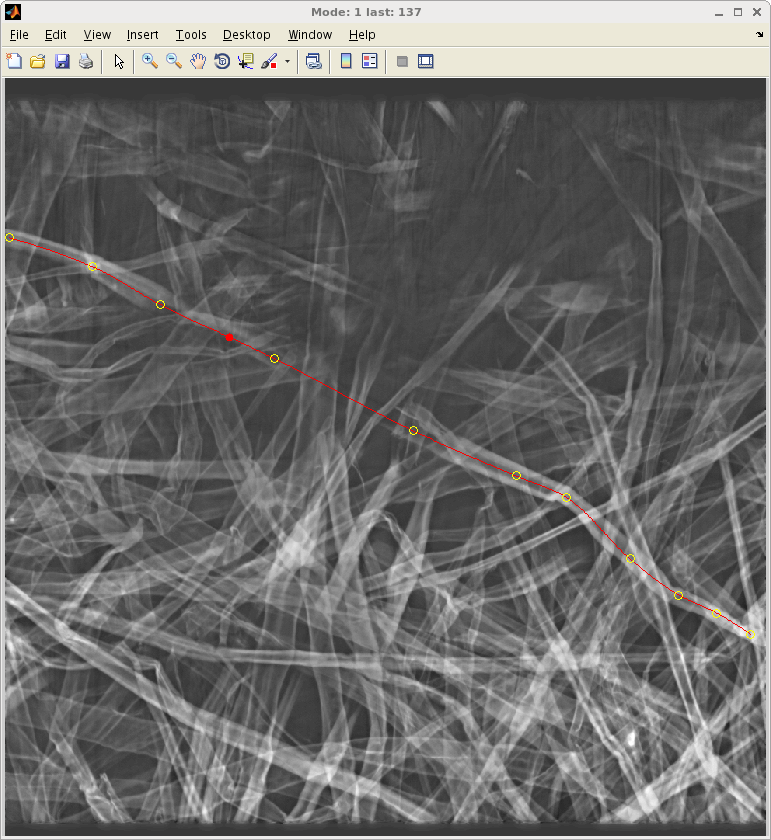
\includegraphics[width=0.48\linewidth]{figures/research/eric.png}
	\caption{\color{red}pending}
	\label{fig:woodseg}
\end{figure*}
%----------------------------------------------------------------------------------------------------------------------------------------------





%----------------------------------------------------------------------------------------------------------------------------------------------

\item
\textbf{Ring Width and Density Profiling with Helical CT}\\
Erik Wernersson, Cris Luengo, Anders Brun, Gunilla Borgefors \\
\ppartners{Jan Van den Bulcke, Dept.~of Forest and Water Management, Ghent University, Belgium}
\ffunding{S-faculty, SLU}
\pperiod{1201 -- 1412}
\aabstract{Dendrochronology relies on accurate measurements of annual ring widths. The most
common method is to use a flatbed scanner to acquire high resolution images of polished wood
surfaces. In this project we investigate potential gains using a helical X-ray device which produces
volume images. Direct advantages include non destructive and simplified sample preparation procedures
as well as compensation for the orientation of the inner structure which can not be seen
with ordinary flatbed scans. It is also possible to find density profiles using the same images.

One article was published in Dendrochronologia 32(1):39-46.}

%---------------------------------------------------------------------------------------------
\item
\textbf{Light scattering in paper}\\
Erik Wernersson, Cris Luengo \\
\ppartners{Tomas Linder and Torbj\"{o}rn L\"{o}fqvist, Lule\r{a} University of Technology, Lule\r{a}}
\ffunding{S-faculty, SLU}
\pperiod{1212 -- 1412}
\aabstract{Fibre orientation is an important structural property in paper and other fibrous materials.
	In this study we explore the relation between light scattering and in-plane fibre orientation
	in paper sheets. Light diffusion from a focused light source is simulated using a
	Monte Carlo technique where parameters describing the paper micro-structure were determined
	from 3D x-ray computed tomography images. Measurements and simulations on both spatially
	resolved reflectance and transmittance light scattering patterns show an elliptical shape
	where the main axis is aligned towards the fibre orientation.
	
	Good qualitative agreement was found at low intensities and the results indicate that
	fibre orientation in thin fibre-based materials can be determined using spatially resolved
	reflectance or transmittance. Published in Optics Express 22(14):16829-16840, 2014.}
%---------------------------------------------------------------------------------------------


\clearpage

%----------------------------------------------------------------------------------------------------------------------------------------------
%----------------------------------------------------------------------------------------------------------------------------------------------
%----------------------------------------------------------------------------------------------------------------------------------------------
%----------------------------------------------------------------------------------------------------------------------------------------------
%----------------------------------------------------------------------------------------------------------------------------------------------

\subsection{Analysis of microscopic biomedical images}

% AAA

\item
\textbf{Identification of Highly Pathogenic Viruses in Transmission Electron Microscopy Images} \label{proj:PVS2}
Gustaf Kylberg, Ida-Maria Sintorn, Ewert Bengtsson, Gunilla Borgefors\\
\ppartner{Vironova AB; Delong Instruments, Brno, Czech Republic; Ali Mirazimi, Kjell-Olof H\"{o}glund, Centre for Microbiological Preparedness; Swedish Institute for Infectious Disease Control (SMI)}
\ffunding{2008--2011 Swedish Civil Contingencies Agency (MSB); Swedish Defense Materiel Administration (FMV); Swedish Agency for Innovative Systems (VINNOVA). 2011--2013 Eurostar project E!6143}
\pperiod{0801--}
\aabstract{This project aims at automating the virus identification process in high resolution TEM images. This, in combination with Project \ref{proj:PVS1} to create a rapid, objective, and user independent virus diagnostic system. The identification task consists of method development for segmenting virus particles with different shapes and sizes and extracting descriptive features of both shape and texture to enable the classification into virus species. Texture features such as variants of Local Binary Patterns and Regional Moments (filter banks constructed from orthogonal moments), are being evaluated on virus textures as well as other texture datasets to get a deeper understanding of the discriminant power of the features under different conditions. A paper comparing, combining and evaluating the discriminating power of local texture descriptors for virus classification was presented at the International Conference on Pattern Recognition (ICPR) in Stockholm in August and Gustaf Kylberg defended his PhD thesis closely linked to this project in March.} 

% BBB

\item
\textbf{The miniTEM Project - Development of a Desk-top TEM with Automated Image Acquisition}\\ \label{proj:PVS1}
Gustaf Kylberg, Ida-Maria Sintorn, Ewert Bengtsson, Gunilla Borgefors\\
\ppartner{Vironova AB; Delong Instruments, Brno, Czech Republic}
\ffunding{Eurostar project E!6143}
\pperiod{1107--1310}
\aabstract{Transmission electron microscopy (TEM) is an important clinical diagnostic and material analysis tool. Transmission electron microscopes are expensive, complex, sensitive and bulky machines, often housed in specially built rooms to avoid vibrations affecting the imaging process. They are to a very large extent manually operated, meaning that an expert in electron microscopy and preferably also in the  application at hand needs to perform the analysis at the microscope, an often very time consuming task. 
	
This project aimed at developing the MiniTEM, a desk-top low voltage TEM designed for imaging biological samples, with a high degree of automation regarding instrument alignment, image acquisition and analysis. The goal was a small, cheap, robust, and easy to use system that requires no more training than any simple lab equipment, and can be hosted in any office or lab (even mobile).
	
Automating the image acquisition process is key for reducing the manual input and making the imaging and analysis more objective. Within the project different strategies for automating the image acquisition were developed and investigated. The first was acquisition of images at random positions on the grid. The second was to search for a specific structure/object and only acquire (store) the images containing the structure/object of interest. The third was similar to the second approach but embedded in a multi-scale approach with the goal to make the acquisition more efficient.
	
The MiniTEM was launched and displayed at the International Microscopy Congress in Prague in September. One instrument was at the conference site and a second piece, physically in Stockholm, was operated remotely from Prague. Abstracts and posters about the project, the developled image analysis methods, and actual instrument, have been presented at various international and national conferences and meetings throughout the year. Gustaf Kylberg successfully defended his PhD thesis early 2014, which was closely linked to this project. The MiniTEM, its GUI and two example images showing a mixture of typical clinical application areas are shown in Figure \ref{fig:miniTEM}.}

\begin{figure}[!h]
	\centering
	
	\subfigure[]{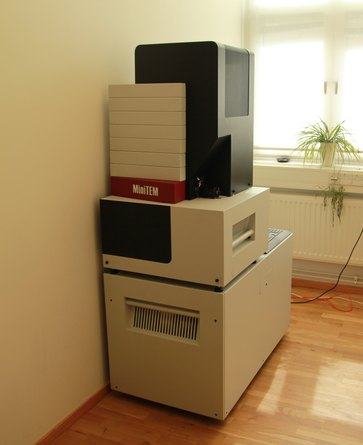
\includegraphics[width=0.4\linewidth]{figures/research/MiniTEM_Instrumentsmallercut.png}}
	\subfigure[]{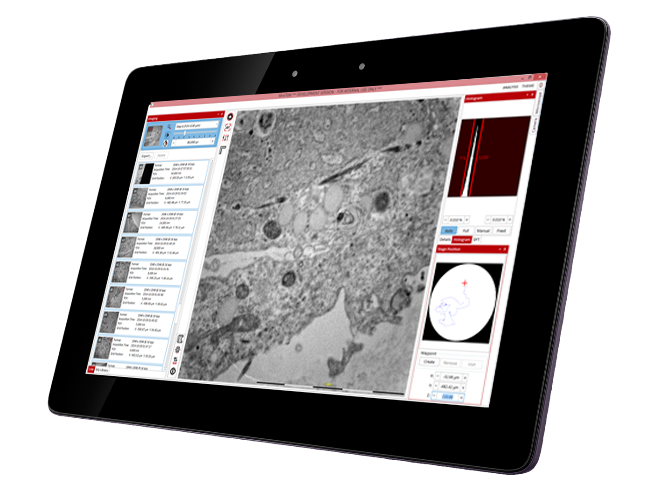
\includegraphics[width=0.4\linewidth]{figures/research/MiniTEMGUIAR2013screenshot.png}}\\
	\subfigure[]{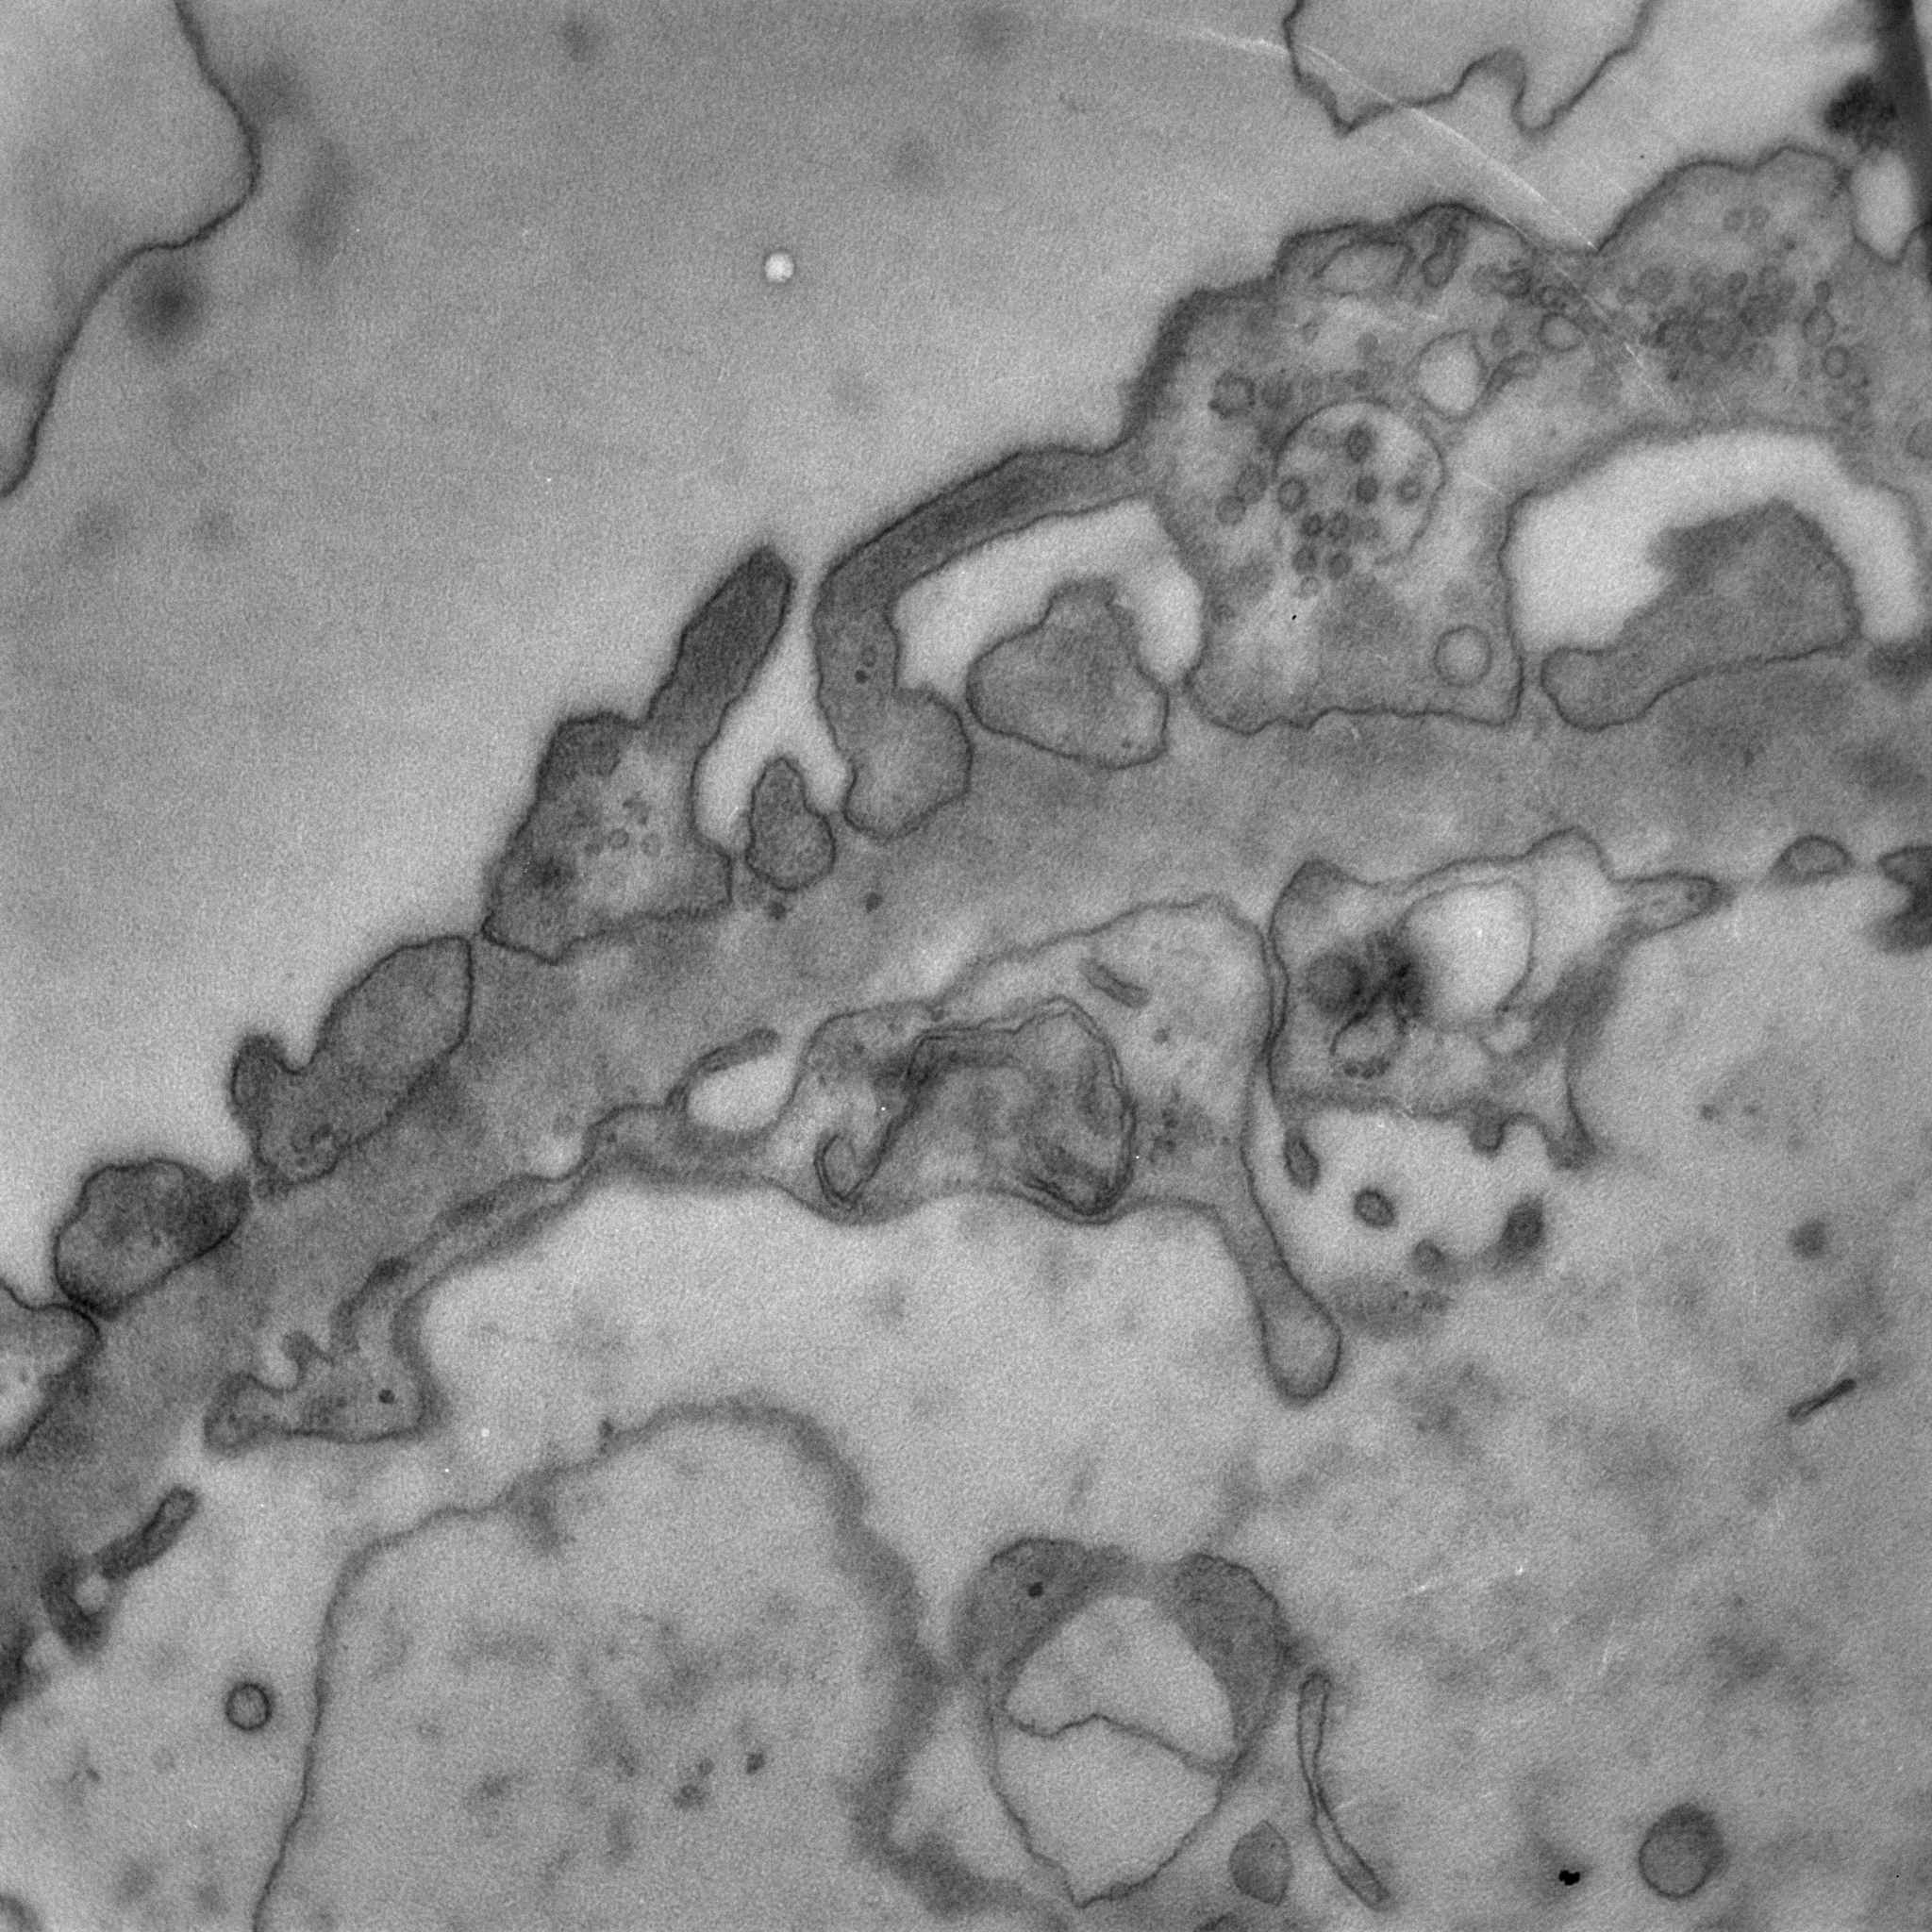
\includegraphics[width=0.4\linewidth]{figures/research/MiniTEMKidneyforAR2013.png}}
	\subfigure[]{\includegraphics[width=0.4\linewidth]{figures/research/MiniTEMAdenoRotaAr2013_FOV500nm.png}}
		\caption{The MiniTEM instruments, its GUI and images of a filtering membrane in a kidney section and a mixture of Adeno and Rota viruses. \label{fig:miniTEM}}
	
	\end{figure}

%\begin{figure*}[!h]
%\centering
%\subfigure[]{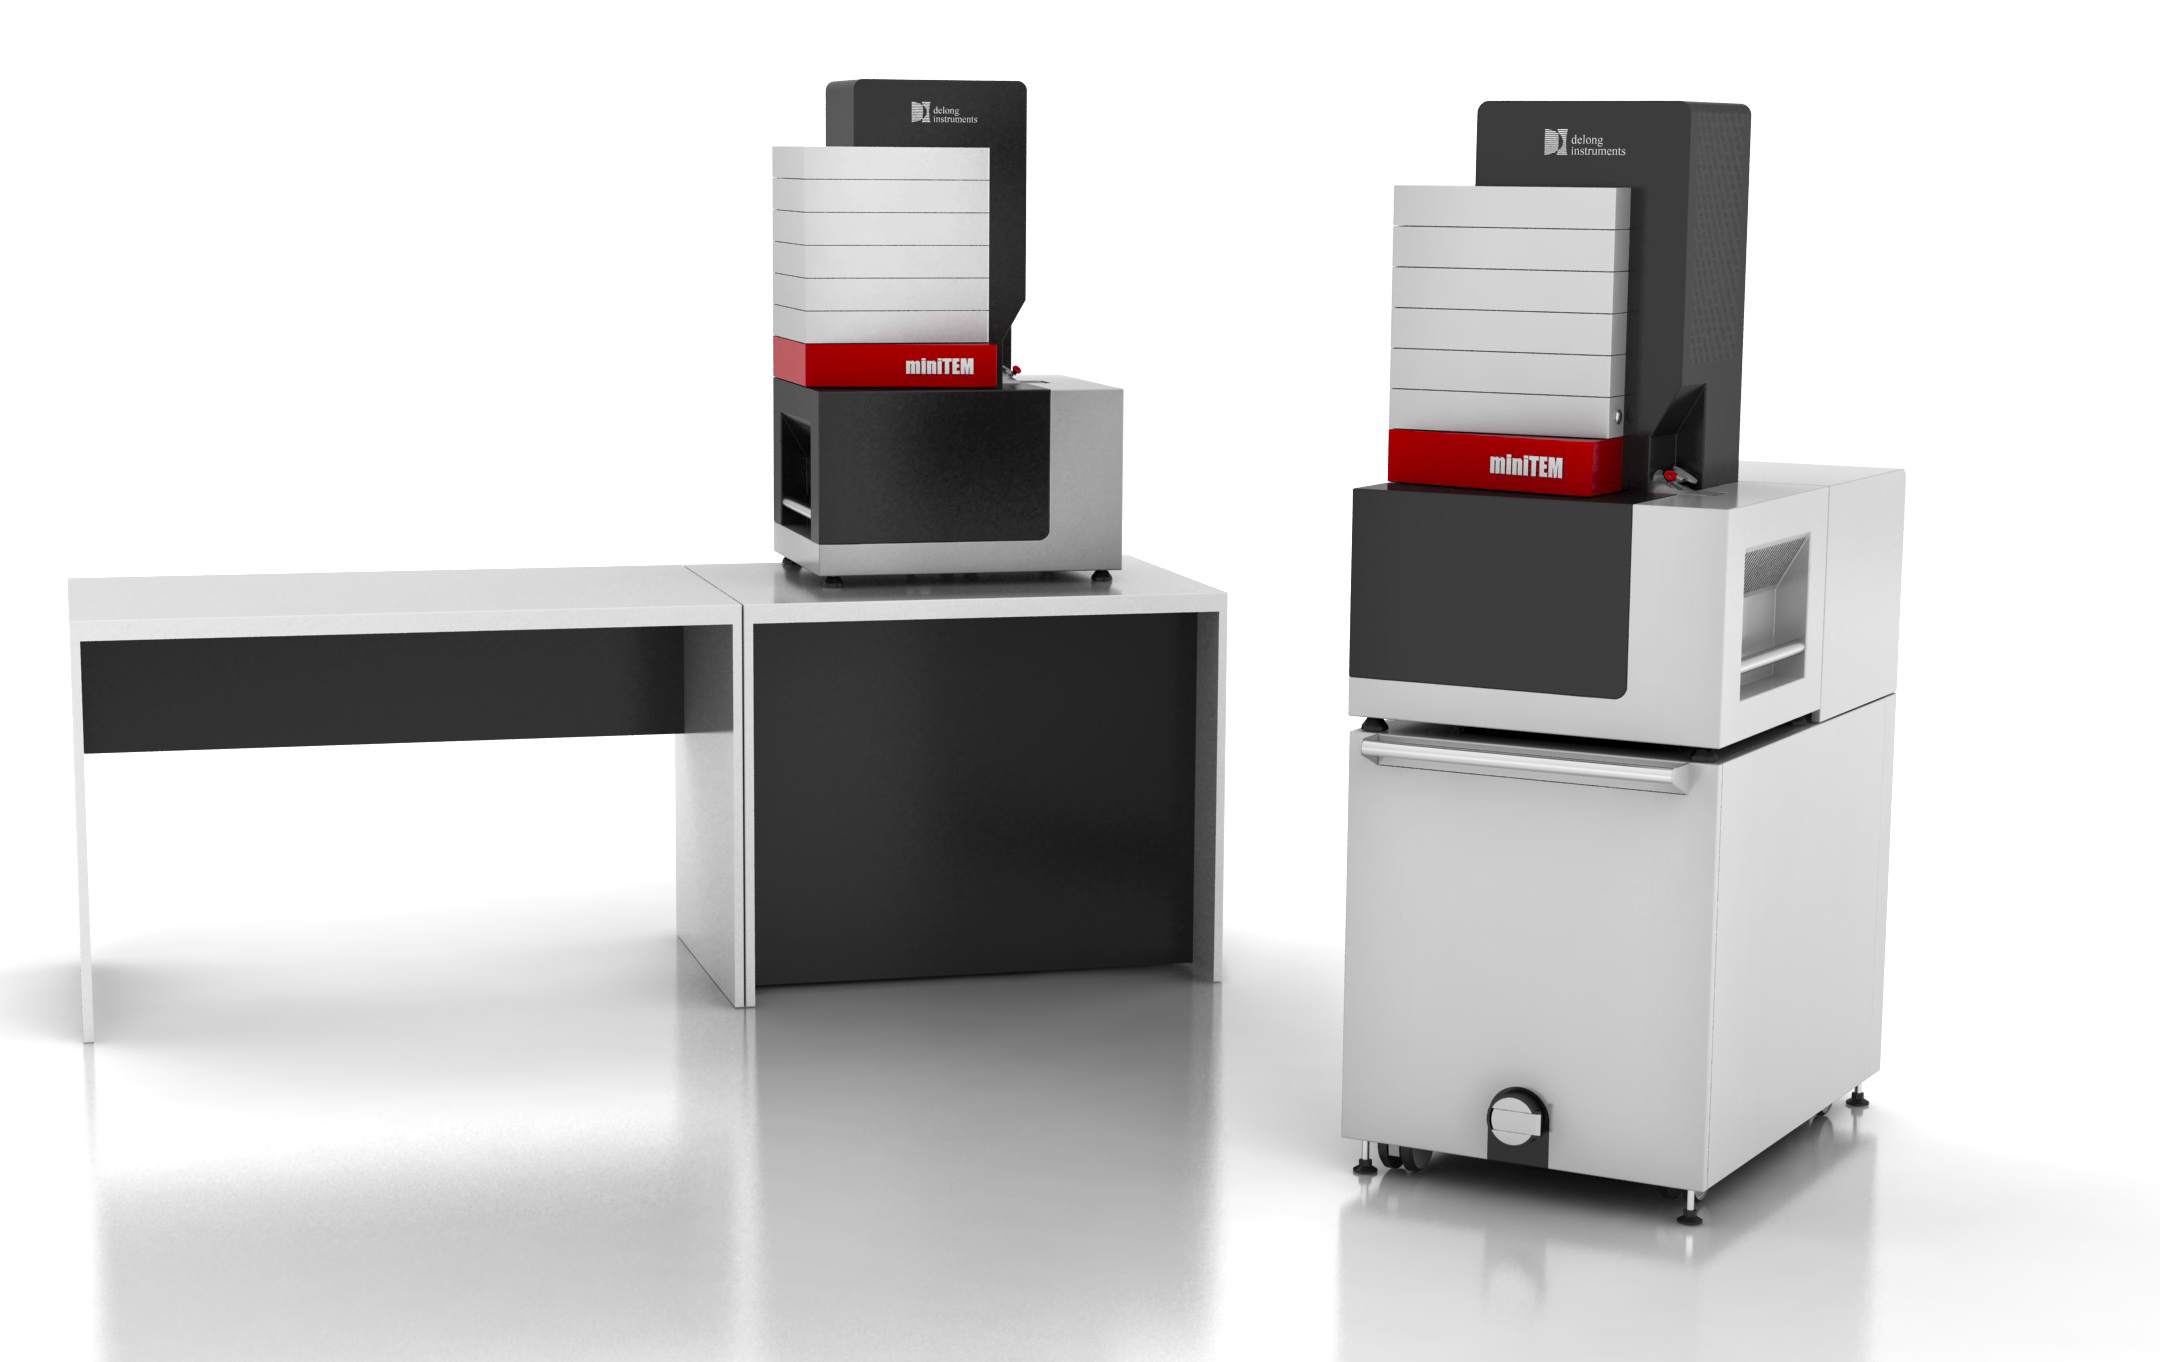
\includegraphics[width=0.36\linewidth]{figures/research/miniTEMLarge.png}}
%\subfigure[]{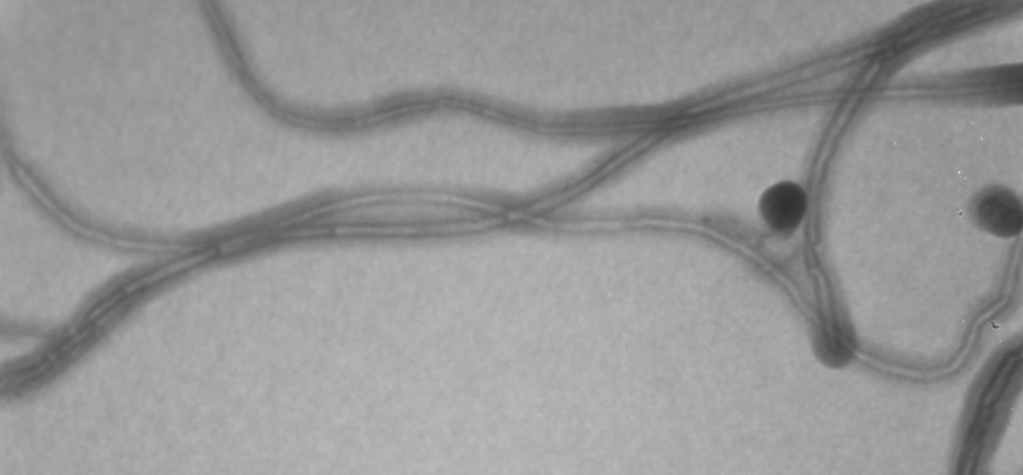
\includegraphics[width=0.48\linewidth]{figures/research/miniTEMnanotubulescutwider.png}}
%\caption{Desk-top and mobile version of the miniTEM (left). Nanotubes, approximately 15nm thick, the first image acquired with the miniTEM (right).}
%\label{fig:miniTEM}
%\end{figure*}

% CCC
\vspace*{-2mm}
\item 
\textbf{\color{red}Detection and Localization of Florescent Signals in STORM Data Using Compressed Sensing}\\
Omer Ishaq, Alexandra Pacureanu, Carolina W\"{a}hlby\\
\ppartners{Johan Elf, Gustaf Ullman, Fredrik Persson, Dept.~of Cell \& Molecular Biology, UU}
\ffunding{SciLifeLab Uppsala, eSSENCE, VR junior researcher grant to CW}
\pperiod{1211-}
\aabstract{Stochastic optical reconstruction microscopy (STORM) is a super-resolution microscopy image acquisition technique for single-molecule localization. Like other stochastic super-resolution microscopy techniques it incorporates a trade-off between spatial- and temporal-resolution. Recently, a compressed-sensing (CS) based variant of STORM, called FasterSTORM, has been developed which substantially increases the temporal sampling of a stack of STORM image frames. This improvement is realized by increasing the density of activated fluorophores in each frame, followed by a subsequent CS-based retrieval of single-molecule positions even with overlapping fluorescent signals.  However, the CS-based retrieval/decoding step is time consuming and can take as much as three hours for each image frame. We have accelerated the FasterSTORM method through parallel processing on multi-core processors. Additionally, we have tested and tried a number of L\raisebox{-.4ex}{\scriptsize 1}-solvers for CS-based recovery of molecule positions. A paper comparing convex and greedy solvers and evaluating the sensitivity of the FasterSTORM to estimation bias of the point spread function (PSF) was submitted to a conference. We are in the process of comparing the performance of the Faster STORM against a wavelet-based approach to localize fluorescent signals in time-lapse images of bacterial cells.}

%DDD

\item 
\textbf{\emph{In Situ} Sequencing of mRNA}\\
Carolina W\"{a}hlby, Alexandra Pacureanu, Petter Ranefall \\
\ppartners{Mats Nilsson, Rongqin Ke, Marco Mignardi, Thomas Hauling, Xiaoyan Qian, SciLifeLab Stockholm/Stockholm University}
\ffunding{SciLifeLab Uppsala; TN-faculty, UU}
\pperiod{1109--}
\aabstract{Profiling of gene expression is prerequisite for understanding the function of cells, organs and organisms, in health and disease. The sequencing techniques currently in use rely on homogenization of the samples. Therefore, the obtained information represents either the average expression profile of the tissue sample or expression profiles of isolated single cells. Our collaborators have developed a new molecular method, enabling \emph{in situ} sequencing of mRNA, so that protein expression can be observed directly in cultured cells or tissue samples. We have developed image analysis tools for automated analysis of sequencing data, mapping, and visualization of gene expression patterns. In 2013 we presented the work as part of a Special Session on Advances in Computer-Aided Histopathology at the IEEE International Symposium on Biomedical Imaging (ISBI), Beijing 2014. The project was also presented at the 1st annual conference for the Society of Biomolecular Imaging and Informatics SBI2, at the JB Martin Conference Center at Harvard Medical School, Boston, MA, USA, where Carolina Wählby was honored with the 'SBI2 President's innovation award' for her presentation on 'Combining image-based \emph{in situ} RNA screening with quantitative analysis of cell and tissue morphology'.}

\begin{figure}[!h]
\centering
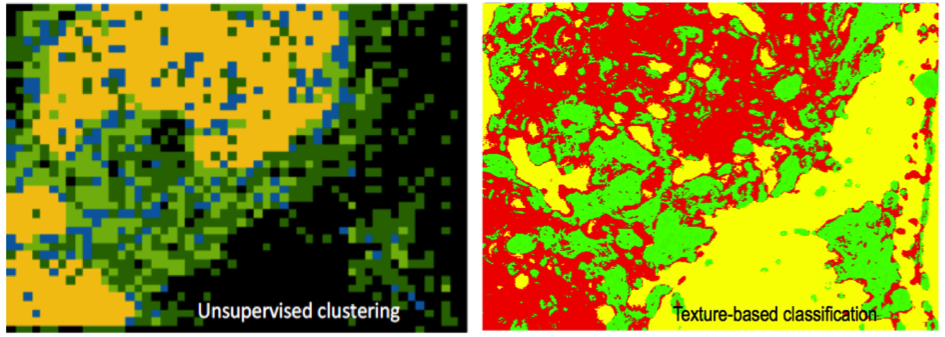
\includegraphics[width=0.85\textwidth]{figures/research/insitumrna.png}
\caption{\label{fig:carolina_insitu} Coupling gene expression to cell and tissue morphology. The gene expression map was divided into patches of $100\times100$ pixels, and patches were clustered by k-means clustering (100 random seeds). The resulting spatial patterns (left) correlate with independent texture-based classification of an H\&E staining of the same tissue sample.} 
\end{figure}

% EEE

\item 
\textbf{Evaluation of the Effect of Compaction Oligonucleotides on the Strength and Integrity of Florescent Signals }\\
Omer Ishaq, Petter Ranefall, Carolina W\"{a}hlby\\
\ppartners{Carl-Magnus Clausson, Linda Andersson, Ola S\"{o}derberg, Dept.~of Immunology, Genetics and Pathology}
\ffunding{SciLife Lab Uppsala}
\pperiod{1310--}
\aabstract{Rolling circle amplification (RCA) performs nucleic acid replication for rapid synthesis of multiple concatenated copies of circular DNA. These molecules can be visually observed through the use of florescent markers. Moreover, the introduction of a compaction oligonucleotide during RCA results in brighter and more compact signals. The project aims to evaluate the effect of compaction oligonucleotides on the strength and integrity of florescent signals. A manuscript has been submitted.}





\item 
\textbf{Skeleton-Based Vascular Segmentation at Interactive Speed} \\
Krist\'{i}na Lidayov\'{a}, Hans Frimmel, Ewert Bengtsson \\
\ppartner{ \"{O}rjan Smedby, Chunliang Wang, Center for Medical Image Science and Visualization (CMIV), Link\"{o}ping University}
\ffunding{VR grant to \"{O}rjan Smedby}
\pperiod{1207--}
\aabstract{Precise segmentation of vascular structures is crucial for studying the effect of stenoses on arterial blood flow. The goal of this project is to develop and evaluate vascular segmentation, which will be fast enough to permit interactive clinical use. The first part is the extraction of the centerline tree (skeleton) from the gray-scale CT image. Later this skeleton is used as a seed region. The method should offer sub-voxel accuracy. 
	
During 2013 we improved the software for fast vessel centerline tree extraction. The method has been tested on several CT data and the results look promissing. Generally main vessel centerlines are detected, but an improvement  needs to be done in order to remove some false positive centerlines. 
	
In year 2014 we improved the software to its final stage. It works on the original Computed Tomography Angiography (CTA) image as the input and produces a node-link representation of the vascular structures for the lower limbs. The method (Figure. \ref{fig:krstinapipeline}) works in two passes: first pass extracts the skeleton of large arteries, and second pass focus on extracting small arteries. Each pass contains three major steps: (1) sets proper intensity ranges for different anatomy structures based on Gaussian curve fitting to the image histogram; (2) apply different filters to detect voxels that are part of arteries, where filters are designed based on intensity and size analysis of ellipse shape on 2-D planes; (3) connect nodes to obtain a centerline tree for the entire vasculature. The method has been tested on 25 CTA scans of the lower limbs (Figure. \ref{fig:krstinacomparison}) and achieved an average of 96\% overlap rate with ground truth. The average computational time is 121 sec/scan.
	
A paper summarizing this work was written and was sent to a Special issue of Pattern Recognition Letters on skeletonization and its applications. At the current stage the paper is under major revision. The work was pressented at SSBA conference and Medicinteknikdagarna.}

\begin{figure}[!htbp]
\centering
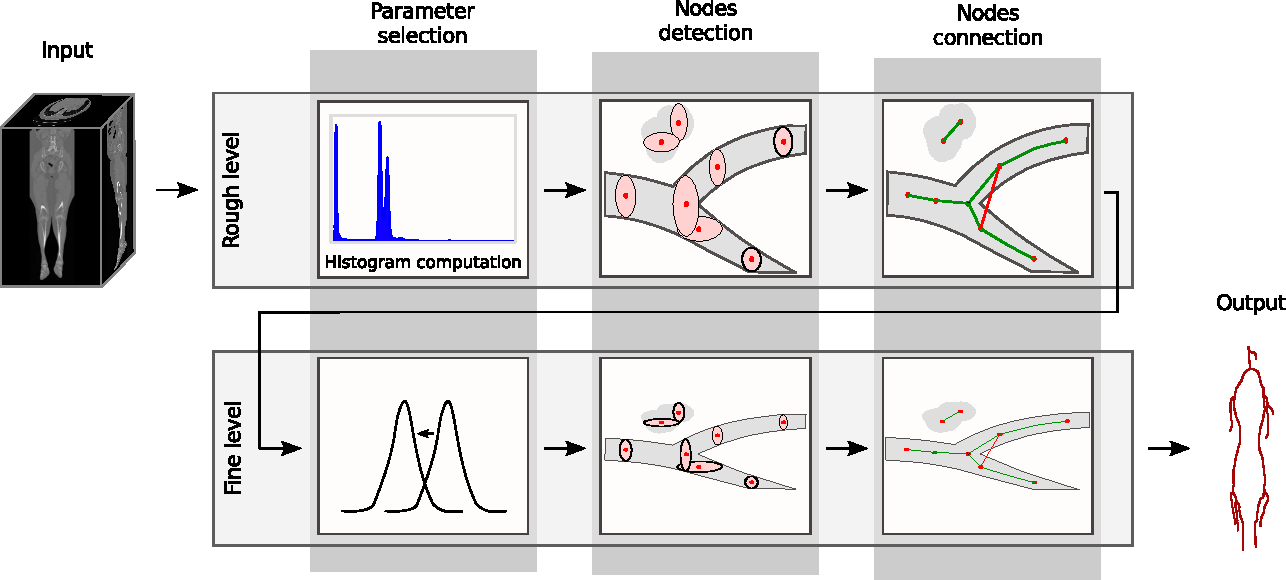
\includegraphics[width=0.7\textwidth]{figures/research/kristinapipeline.pdf}
\caption{Flow chart of the proposed method}
\label{fig:krstinapipeline} 

\end{figure}

\begin{figure}[!htbp]
	\centering
	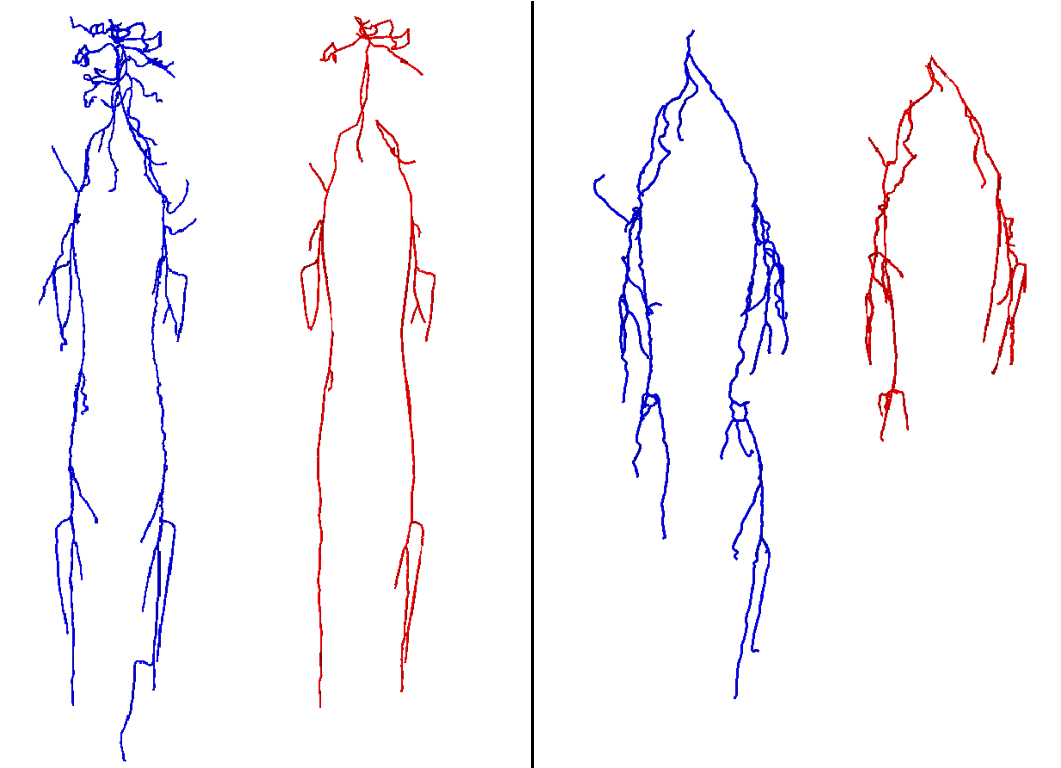
\includegraphics[width=0.7\textwidth]{figures/research/kristinacomparison.pdf}
	\caption{Ground truth skeleton in blue colour and resulting skeleton in red colour are shown for two cases from a clinical routine. The case on the right side contains an occluded segment in the femoral artery and severe stenoses.} 
	\label{fig:krstinacomparison}
\end{figure}





% GGG
\newpage

\item
\label{proj:stemcells}
\textbf{SciLifeLab Cancer Stem Cell Program}\\
Damian Matuszewski,Carolina W\"{a}hlby, Ida-Maria Sintorn\\
\ppartners{Sven Nelander, Karin Forsberg-Nilsson, Irina Alafuzoff, Ulf Landegren, Anna Segerman, Tobias Sj\"{o}blom, Lene Urborn and Bengt Westermark, Department of Immunology, Genetics and Pathology and SciLifeLab, UU, Bo Lundgres, the Karolinska Institute and SciLifeLab, Stockholm, Rebecka J\"{o}rnsten, Chalmers, Gothenburg, and G\"{o}ran Hesselager, UU Hospital, Uppsala}
\ffunding{AstraZeneca-Science for Life Laboratory Joint Research Program}
\pperiod{1303--}
\aabstract{The SciLifeLab Cancer Stem Cell Program is a cross-platform initiative to characterize cancer stem cells (CSCs). Previously, the development of drugs targeting the CSC population in solid tumors has been curbed by the lack of valid cell model systems, and the complex genetic heterogeneity across tumors, factors that make it hard to assess new targets or predict drug responses in the individual patient. To solve these problems, our aim is to develop a biobank of highly characterized CSC cultures as a valid model of cancer heterogeneity. We will combine mathematical and experimental approaches, including image-based high-throughput cell screening, to define the spectrum of therapeutically relevant regulatory differences between patients. This will help elucidate mechanisms of action and enable accurate targeting of disease subgroups. During 2013-2014, patient data was collected, and a number of primary cell lines were established. Cultured cells were exposed to a different treatments and doses (more than 2500 different treatments per cell line), and imaged by fluorescence as well as bright-field microscopy, and current focus is on extracting meaningful morphological descriptors from the image data. 
Developed tools are also applied in a cell cycle analysis project realized together with Jordi Carreras Puigvert, the Karolinska Institute and SciLifeLab, Stockholm.}


\begin{figure}[!htbp]
	\centering
	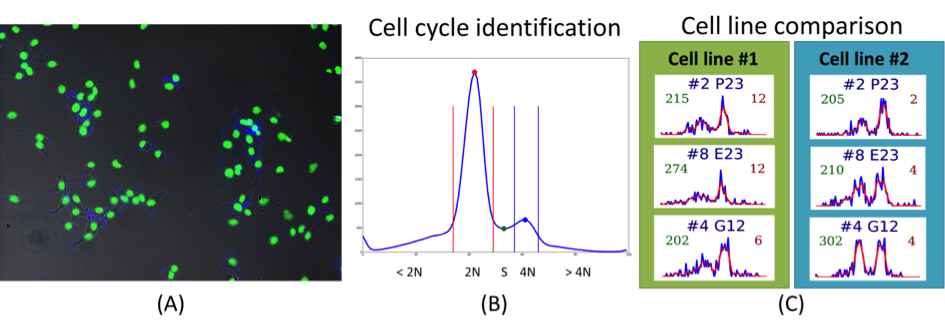
\includegraphics[width=0.85\textwidth]{figures/research/stemcell.png}
	\caption{(A) Sample cancer stem cells image. Figures (B) and (C) present histograms of one of the automatically extracted features – DNA content per cell. (B) The different phases of the cell cycle can be identified based on the DNA content in negative control cells, by assuming that cells spend the majority of their time with either two (2N phase) or four (4N phase) copies of the DNA. Cells from different cell lines respond in a slightly different way to the same drug treatments, and (C) shows DNA histograms for treatments that arrest part of the cell population in the 4N phase.} 
	\label{fig:stemcell}
\end{figure}



%HHH

\item \textbf{Endothelial Cell Segmentation of the Cornea of Human Eyes}\\
Bettina Selig, Cris Luengo\\
\ppartners{Bernd Rieger, Quantitative Imaging Group, Delft University
of Technology, Netherlands; Koen Vermeer, The Rotterdam Eye Hospital, The Netherlands}
\ffunding{S-faculty, SLU}
\pperiod{1103--}
\aabstract{The corneal endothelium plays a key role in maintaining the transparency of the cornea.Because the cells in the endothelium do not regenerate, the cell density decreases with age; this reduces its ability to maintain the processes needed to keep the cornea transparent. Thus, being able to measure this density in patients is very important. The endothelium can be imaged by specular microscopy or by confocal scanners, and measurements can be obtained manually, automatically with manual corrections, or fully automatically with current software (e.g., Nidek's NAVIS). Unfortunately, the results of the automatic methods are often useless, especially at low cell densities. Together with the Rotterdam Eye Hospital, we have developed a fully automatic method to segment individual cells in the corneal endothelium. The result of the method can be used to determine the cell density, but also other parameters of interest, like pleomorphism (cell shape) and polymegathism (cell size variation). Our segmentation method produces a segmentation that matches a manual segmentation reasonably well, for a wide range of cell densities and image qualities. These results have been submitted for publication during 2014.}



%%% III

\item \textbf{CerviScan}\\
Ewert Bengtsson, Patrik Malm, Bo Nordin\\
\ppartners{Rajesh Kumar, Centre for Development of Advanced Computing (CDAC), Thiruvananthapuram, Kerala, India; K. Sujathan, Regional Cancer Centre, Thiruvananthapuram, Kerala, India; Andrew Mehnert, Chalmers}
\ffunding{Swedish Governmental Agency for Innovation Systems (VINNOVA); Swedish Research Council; SIDA}
\pperiod{0801--}
\aabstract{Cervical cancer is a disease that annually kills over a quarter of a million women world-wide. This number could be substantially reduced if women were regularly screened for signs of cancer precursors using the well-established Pap-test. If detected early, these precursors can be treated with a very high rate of success. A problem with the Pap-test is that it requires highly trained cytotechnologists to perform the time consuming visual analysis of the specimen. For over 50 years attempts to automate this process have been made but still no cost effective systems are available.
	
The CerviScan project is an initiative from the Indian government, managed by the research institute CDAC in cooperation with the Regional Cancer Centre (RCC) in Kerala and CBA in Sweden, aimed at creating a low cost, automated screening system. The system will reduce the number of cytotechnologists needed for population screening by identifying and removing specimen that are clearly normal. A prototype system has been created and used to screen over 1000 specimen. Initial classification results are promising but screening times are still about 10 times longer than what is realistic in a real screening setting. Plans for the next phase of the project, focusing on dedicated hardware, are awaiting the result of a funding application in India.
 
A subproject on developing improved ways of describing the nuclear chromatin patterns based on new image analysis methods has been spun off and is describe as project XX ({\color{red}Advanced methods for reliable and cost efficient image processing in life sciences})

The project has resulted in several recent publications and a PhD thesis: "Image Analysis in Support of Computer-Assisted Cervical Cancer Screening" which was defended February 7, 2014 by Patrik Malm.
}


%\newpage

%JJJ

\item \textbf{Automated Tissue Image Analysis using Pattern Recognition}\\
Jimmy Azar, Anders Hast, Ewert Bengtsson  \\
\ffunding{TN-faculty, UU}
\pperiod{1001--1410}
\aabstract{The research was initially part of a VR supported project for grading of prostate cancer. The final part of the research which took place during 2013-2014 extended this to more general ways of describing the architecture of histological tissues.
	 
Immunohistochemistry can facilitate the quantification of biomarkers such as estrogen, progesterone, and the human epidermal growth factor 2 receptors, in addition to Ki-67 proteins that are associated with cell growth and proliferation. We developed a method for the identification of paired antibodies based on correlating probability maps of immunostaining patterns across adjacent tissue sections. Samples from the Human Protein Atlas project were used to test the method.

We also developed a new feature descriptor for characterizing glandular structure and tissue architecture, which form an important component of Gleason and tubule-based Elston grading. The method is based on defining shape-preserving, neighborhood annuli around lumen regions. 

These two studies were accepted as journal papers. They also became part of the PhD thesis by Jimmy Azar, with the same title as the project, defended on October 10 2014.}





% NNN

\item 
\textbf{Segmentation and Tracking of E.coli Bacteria in Bright-Field Microscopy Images}\\
Sajith Kecheril Sadanandan, Carolina W\"{a}hlby\\
\ppartners{Johan Elf and David Fange and Alexis Boucharin, Dept.~of Cell \& Molecular Biology, UU}
\ffunding{SciLifeLab Uppsala, eSSENCE, VR junior researcher grant to CW}
\pperiod{1210--}
\aabstract{Live cell experiments pave way to understand the complex biological functions of living organisms. Most live cell experiments require monitoring of cells under different conditions over several generations. The biological experiments display wide variations even when performed under similar conditions, and therefore need to include large population studied over several generations to provide statistically verifiable conclusions. Time-lapse images of such experiments usually generate large quantities of data, which become extremely difficult for human observers to evaluate. Thus, automated systems are helpful to analysis of such data and provide valuable inference from the experiment. In this work we segment and track E. coli bacteria cells over time. We developed a novel segmentation method, which is fast and robust in delineating bacterial cells in phase contrast microscopy images. The preliminary results (Figure \ref{fig:ecoliseg}) were presented as poster at the international Bioimage Informatics 2014 conference in Leuven, Belgium.}

\begin{figure}[!htbp]
	\centering
	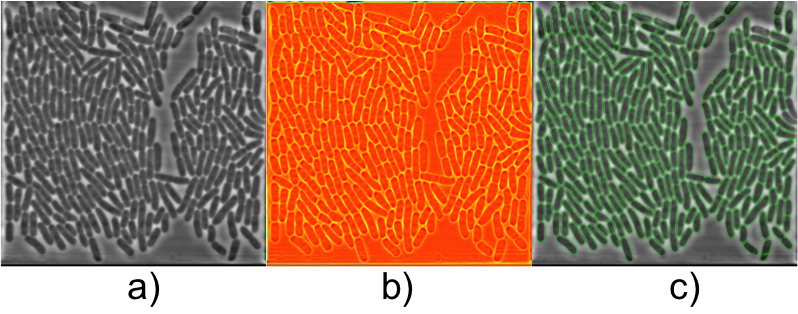
\includegraphics[width=0.85\textwidth]{figures/research/ecoliseg.png}
	\caption{a) Input phase contrast image of E. coli bacteria, b) contrast enhanced image, c) segmentation result overlaid on the input image.} 
	\label{fig:ecoliseg}
\end{figure}



%OOO

\item % Analysis of microscopic biomedical images
\label{proj:cellsurfaceDiffusion}
\textbf{Modelling Diffusion on Cell Surfaces}\\
Ida-Maria Sintorn, Robin Strand \\
\ppartners{Ingela Parmryd, Dept.~of Medical Cell Biology, UU; Jeremy Adler, Dept.~Of Immunology, Genetics and Pathology, UU}
\ffunding{TN-faculty, UU; S-faculty, SLU; VINNMER programme, Swedish Governmental Agency for Innovation Systems}
\pperiod{1101--}
\aabstract{A cell surface is a highly irregular and rough. The surface topography is however usually ignored in current models of the
	plasma membrane, which are based on 2D observations of diffusion that really occurs in 3D. In this project we model diffusion on
	non-flat surfaces to explain biological processes occurring on the cellsurface. }

%PPP

\item 
\textbf{Analysis of Male Reproductive Tract Morphology in Reproductive Toxicology}\\
Azadeh Fakhrzadeh, Cris Luengo, Gunilla Borgefors\\
\ppartners{Ellinor Sp\"{o}rndly-Nees,  Lena Holm, Dept.~of Anatomy, Physiology and Biochemistry, SLU}
\ffunding{SLU (KoN)}
\pperiod{1009--}
\aabstract{Reproductive toxicology is the study of chemicals and their effects on the reproductive system of humans and animals. In reproductive toxicology, there is a strong need to detect structural differences in organs that often have both a complex microscopic structure and function. This problem is further complicated because standard techniques are based on the examination of two-dimensional sections of a three-dimensional structure. The aim of this project is to develop methods to objectively describe microscopic structures of male reproductive organs and to test these in reproductive toxicology research. The project is comparative and  includes studies of organs from rooster and mink. We are developing automatic and interactive methods to analyze the relevant structures in the histology images of testis. We have constructed a semi-automatic method to delineate the epithelium cell layer in testicular tissue.
The cell nuclei are detected using the fast radial symmetry filter. A graph is constructed on top of the epithelial cells (Fig. \ref{testis}). Graph-cut optimization method is used to cut the links between cells of different tubules. Generating sperms in seminiferous tubules is a cyclic process, during which various generations of germ cells in epithelial layer undergo a series of developmental steps. This cycle can be subdivided into 12 different stages. We are currently developing a texture-based classification method to determine each tubule's stage.}

\begin{figure}[h]
\centering %\scalebox{1}{}
\includegraphics[width=0.8\textwidth]{figures/research/M1001cut.png}
 \caption{A graph constructed on top of Gata-4 marked germ cells.}
 \label{testis}
 \end{figure}

%QQQ

\item 
\textbf{Automated Classification of Immunostaining Patterns in Breast Tissue from the Human Protein Atlas}\\
Andreas K{\aa}rsn\"{a}s, Martin Simonsson, Carolina W\"{a}hlby, Robin Strand\\
\ppartners{Caroline Kampf, The Human Protein Atlas (HPA); Virginie Uhlmann,  Imaging Platform, Broad Institute of Harvard and MIT, Cambridge, Massachusetts MA, USA; S. Issac Niwas, P. Palanisamy, Dept.~of ECE, National Institute of Technology (NIT), Tiruchirappalli, India}
\ffunding{SciLifeLab Uppsala}
\pperiod{1201-1303}
\aabstract{The Human Protein Atlas (HPA) is an effort to map the location of all human proteins (\url{http://www.proteinatlas.org/}) and contains a large number of histological images of sections from human tissue. Methods for quantification of staining patterns in histopathology have many applications, ranging from antibody quality control to tumor grading. In this project we have tested a new method based on complex wavelets textural features as well as an approach inspired by WNDCHARM (Weighted Neighbor Distances using a Compound Hierarchy of Algorithms Representing Morphology) for classifying nuclear versus cytoplasmic staining. During 2013, a paper was published in Journal of Pathology Informatics.}

%RRR

\item % Analysis of microscopic biomedical images
\label{proj:CombatingCancer}
\textbf{Combating Breast Cancer by Digital Pathology}\\
Andreas K{\aa}rsn\"{a}s, Robin Strand, Carolina W\"{a}hlby, Ewert Bengtsson\\
\ppartners{Visiopharm, H{\o}rsholm, Denmark; Clinical Pathology Division, Vejle hospital, Vejle, Denmark}
\ffunding{NordForsk Private Public Partnership PhD Programme and Visiopharm}
\pperiod{0909--}
\aabstract{The results of analyses of tissue biopsies by pathologists are crucial for breast cancer patients. In particular, the precision of a patient's prognosis, and the ability to predict the consequences of various treatment opportunities before actually exposing the cancer patient, depend on the detection and quantification of biomarkers in tissue sections by microscopy. Experience from the last decade has revealed that manual detection and quantification of biomarkers by microscopy of tissue biopsies is highly dependent on the competencies and stamina of the individual pathologist. The aim of the present PhD project is to develop software-based algorithms that can facilitate the workflow and ensure objective and more precise results of the quantitative microscopy procedures in breast cancer.

During 2012, we worked on a project for verifying antibodies by comparing staining patterns in immune-stained histological images. The project was made in collaboration with the Human Protein Atlas project. We made a comparison of different methods for classifying staining patterns in histology. This work was presented at MICCAI'12 in Nice. We also presented the \textit{vectorial minimum barrier distance}, a new method for computing gray-weighted distance transforms while incorporating vectorial data, at ICPR'12 in Tsukuba, Japan. 

Early 2013, we started a new project aimed at developing a new method for registering histological images of consecutive sections with different staining. The project resulted in an article about multimodal registration using locally rigid transforms. The article is currently under review. In 2013, we also finished a journal article presenting a histopathological tool for sub-cellular quantification. The article was accepted early 2014 for publication in the journal \textit{Computer methods in Biomechanics and Biomedical Engineering: Imaging \& Visualization.}}

%SSS

\item 
\textbf{Automatic, Quantitative Malignancy Grading of Prostate Cancer using Image Analysis}\\
Ingrid Carlbom, Christophe Avenel\\
\ppartners{Christer Busch and Anna Tolf, Department of Immunology, Genetics and Pathology, University Hospital}
\ffunding{The Swedish Research Council, Hillevi Fries Research Fund}
\pperiod{1001--}
\aabstract{Gleason grading is the most widely used system for determining the severity of prostate cancer. The Gleason grade is determined visually under a microscope from prostate tissue that is most often stained with Hematoxylin-Eosin (H\&E).

\begin{figure}[!htbp]
\centering
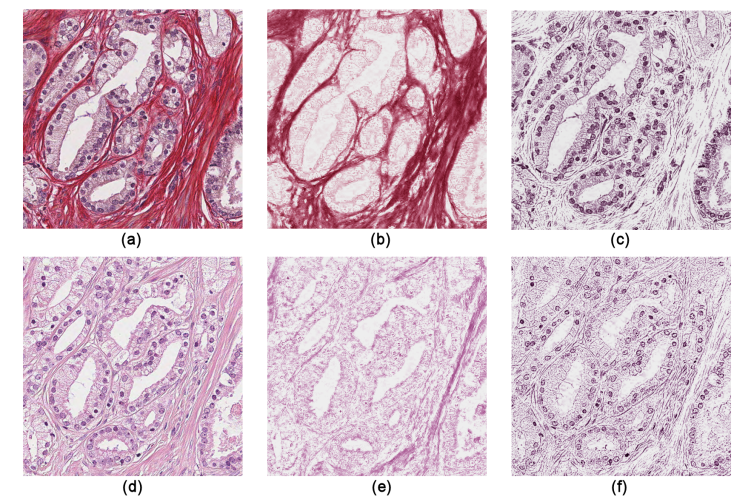
\includegraphics[width=.95\textwidth]{figures/research/prostate2.png}
\caption{Results of color decomposition: (a) original tissue image stained with Sir-Htx, (b) stroma density map, and (c) epithelial density map; (d) original tissue image stained with H\&E, (e) stroma density map, and (f) nuclei density map. \label{fig:prostate2}}
\end{figure}

\textit{Stain for blind color decomposition} In an earlier study we demonstrated that H\&E is not ideal for machine learning applications, but that other stains, such as Sirius-hematoxylin (Sir-Htx), may perform better. This year we demonstrated the advantages of this stain over H\&E for blind color decomposition (Fig. \ref{fig:prostate2}). When compared to ground truth defined by an experienced pathologist, the relative root-mean-square errors of the color decomposition mixing matrices for Sir-Htx are better than those for H\&E by a factor of two, and the Pearson correlation coefficients of the density maps resulting from the decomposition of Sir-Htx-stained tissue gives a 99\% correlation with the ground truth. Qualitative examples of the density maps confirm the quantitative findings and illustrate that the density maps will allow accurate segmentation of morphological features that determine the Gleason grade.
\newpage
\textit{Identification of epithelial nuclei} From the epithelial density map, resulting from the blind color decomposition of Sir-Htx-stained prostate tissue, we used a marked point process to segment the epithelial nuclei (Fig. \ref{fig:prostate3}). This enables us to extract nuclei as individual, joint, or overlapping objects generally without discarding overlapping parts and therefore without major loss in segmentation precision. The algorithm, which was originally developed for breast cancer tissue nuclei identification, uses simulated annealing combined with a "birth and death" process to find the best match with the density map, and was adapted to prostate tissue by pre-and-post processing methods.

\textit{Database of images from whole mount sections} We have created two online tools in order to build a database of graded images. The image selection tool is based on OpenSeaDragon (an open-source, web-based viewer for zoomable images) and facilitates the selection of small images from whole mount sections. With this tool we are building an image database where each image has a dominant pattern that represents for example one Gleason grade, benign tissue, stroma, or artifacts such as a tear in the tissue. The grading tool allows multiple pathologists to grade and comment on the previously selected images, without seeing each other grades, and is a basis for a consensus-graded database for developing and testing automatic Gleason grading algorithms (Fig. \ref{fig:prostate4}).} 

\begin{figure}
\centering
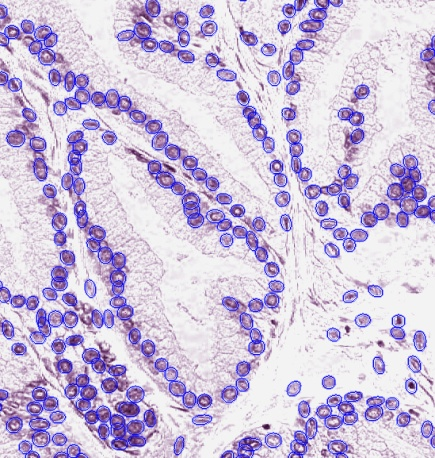
\includegraphics[width=.5\textwidth]{figures/research/prostate3.jpg}
\caption{Epithelial nuclei identified by the marked point process. \label{fig:prostate3}}
\end{figure}

\begin{figure}
\centering
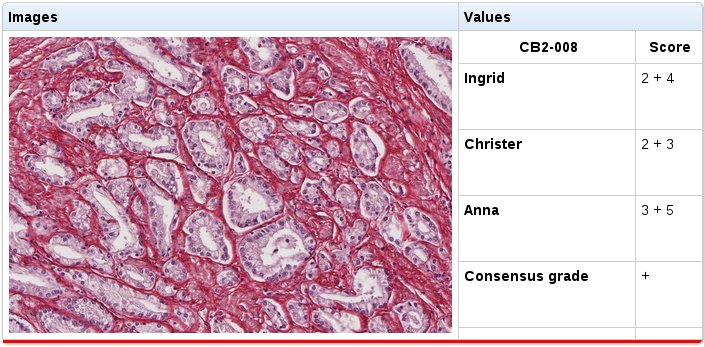
\includegraphics[width=.9\textwidth]{figures/research/prostate4.jpg}
\caption{Example of a sub-section of a whole-mount tissue section with three individual scores. \label{fig:prostate4}}
\end{figure}

%TTT
\newpage

\item 
\textbf{Automated Quantification of Zebrafish Tail Deformation for High-throughput Drug Screening}\\
Omer Ishaq, Alexandra Pacureanu, Carolina W\"{a}hlby\\
\ppartners{Joseph Negri, Mark-Anthony Bray, Randall T. Peterson, Broad Institute of Harvard and MIT}
\ffunding{SciLifeLab Uppsala}
\pperiod{1203--1304}
\aabstract{Zebrafish (\emph{Danio rerio}) is an important model organism in biomedical research due to its ease of handling and translucent body and consequently many human disease models have been established in the Zebrafish. Zebrafish embryos undergo spinal deformation upon exposure to chemical agents, such as Camptothecin (Cpt), that inhibit DNA repair. We are developing automated image-based quantification of spine deformation enabling whole-organism based assays for use in early-phase drug discovery campaigns. Our automated method for accurate high-throughput measurement of tail deformations in multi-fish micro-plate wells generates refined medial representations of partial tail-segments. Subsequently, these disjoint segments are analyzed and fused to generate complete Zebrafish tails (Fig. \ref{fig::zebrafish_curvature}). Based on these estimated tail curvatures we reach a classification accuracy of 91\% on individual animals as compared to known control treatment. This accuracy is increased to 95\% when combining scores for fish in the same well. A paper describing the methods and results was published and presented at the International Symposium for Biomedical Imaging (ISBI) in April 2013.}

\begin{figure*}[!htbp]
\centering
\subfigure[]{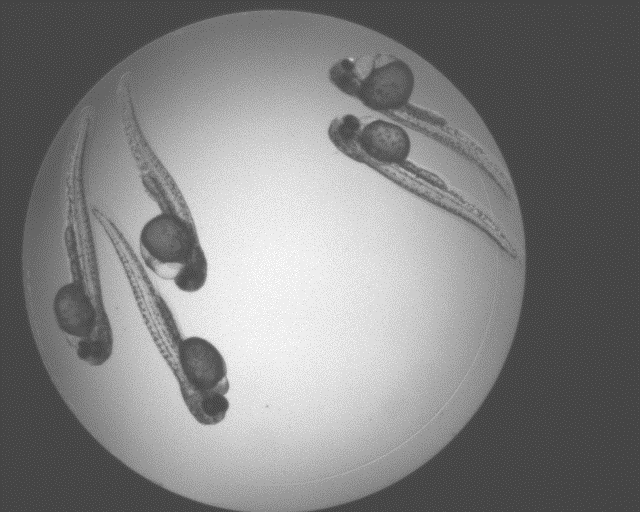
\includegraphics[width=0.3\textwidth]{figures/research/curvature1.png}}
\subfigure[]{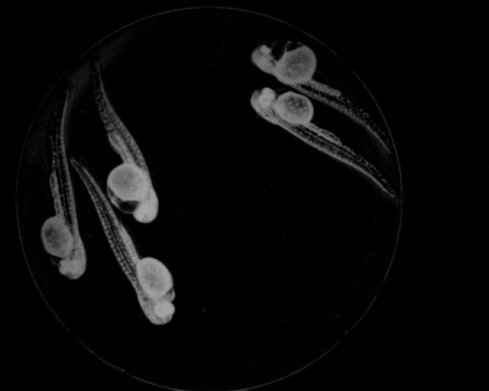
\includegraphics[width=0.3\textwidth]{figures/research/curvature2.png}}
\subfigure[]{
\includegraphics[width=0.3\textwidth]{figures/research/curvature3.png}}

\subfigure[]{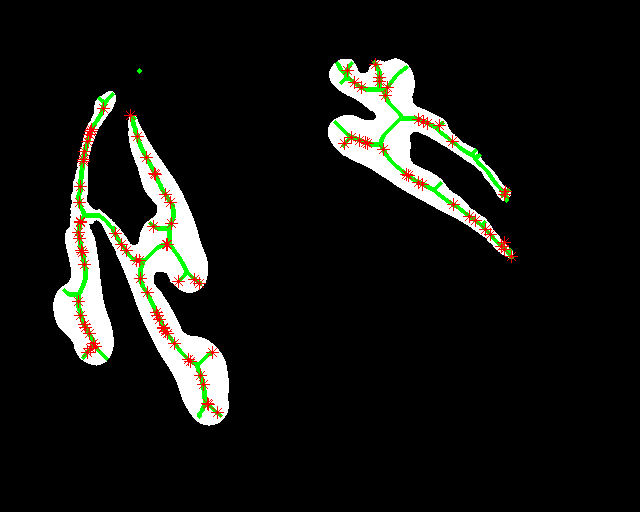
\includegraphics[width=0.3\textwidth]{figures/research/curvature4.png}}
\subfigure[]{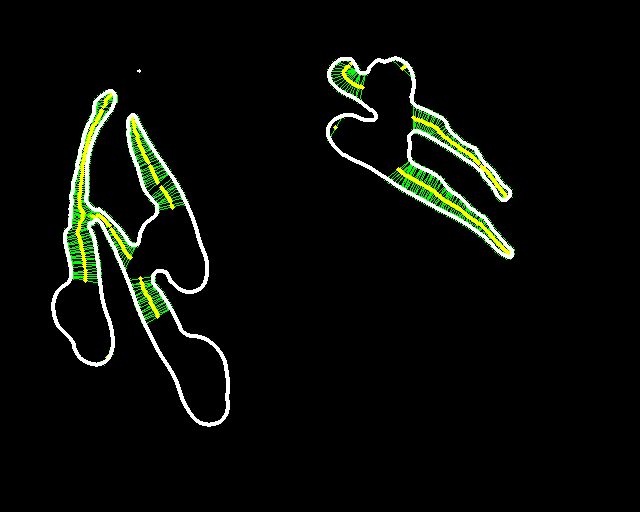
\includegraphics[width=0.3\textwidth]{figures/research/curvature5.png}}
\subfigure[]{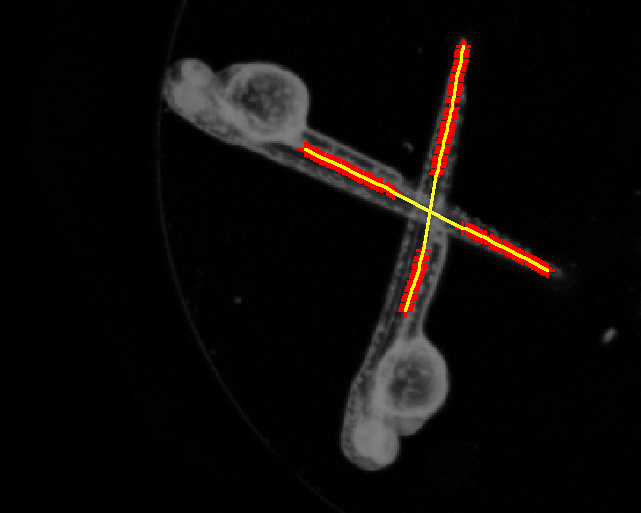
\includegraphics[width=0.3\textwidth]{figures/research/curvature6.png}}
\caption{Steps for curvature extraction: (a) An input image; (b) After illumination correction; (c) Binary image after smoothing and thresholding; (d) Computed medial axes (highlighted in green) and seed-points (highlighted in red); (e) Refined medial axes (highlighted in yellow); (f) Medial axis fusion: the red lines represent tail-segments fused together to yield the complete tails (shown in yellow).}
\label{fig::zebrafish_curvature}
\end{figure*}

%UUU

\item 
\textbf{Quantification of Zebrafish Lipid Droplets}\\
Petter Ranefall, Carolina W\"{a}hlby\\
\ppartners{Marcel den Hoed, Manoj Bandaru, Erik Ingelsson, Department of Medical Sciences and SciLifeLab, UU}
\ffunding{SciLifeLab Uppsala}
\pperiod{1308--}
\aabstract{The aim of this project is to identify novel targets for the therapeutic intervention of coronary artery disease. This is done by following-up results from genome-wide association studies in epidemiological studies using a zebrafish model system.  Using image analysis we try to identify and characterize causal genes within loci that have so far been identified as associated with coronary heart disease by (high-throughput) screening of atherogenic processes in wildtype and mutant zebrafish, both before and after feeding on a control diet or a diet high in cholesterol. Using confocal microscopy we can image fat accumulation in the zebrafish (Fig. \ref{fig:hamid}).}

\begin{figure}[!htbp]
\centering
\subfigure[]{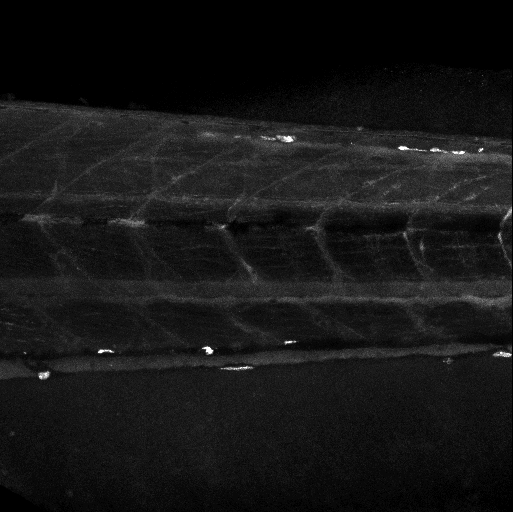
\includegraphics[width=44mm,height=44mm]{figures/research/lipid1.png}}
\subfigure[]{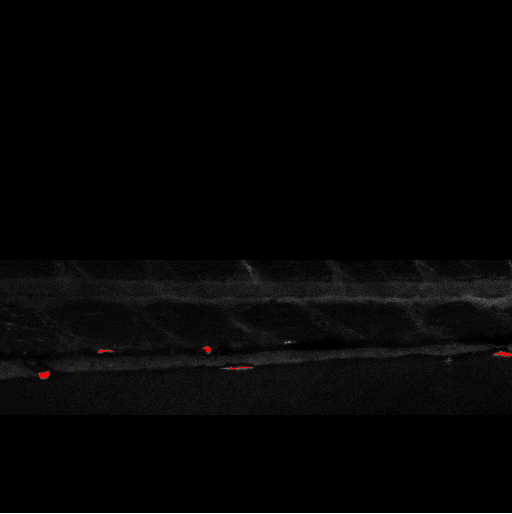
\includegraphics[width=44mm,height=44mm]{figures/research/lipid2.png}}
\caption{\label{fig:hamid}
The image to the left is a maximum projection of the zebrafish image volume, and the image to the right shows the detected stationary lipids in red.}
\end{figure}

%VVV

\item \textbf{Optical Projection Tomography}\\
Alexandra Pacureanu, Omer Ishaq, Carolina W\"{a}hlby\\
\ppartners{Amin Allalou, Izolde AB, Uppsala; Johan Ledin, Evolutionary Biology Centre, Zebrafish platform, SciLifeLab Uppsala; Jos Buijs, Ridgeview Uppsala, Carlos Pardo, Mehmet F. Yanik, Research Laboratory of Electronics, Massachusetts Institute of Technology, Cambridge, USA}
\ffunding{SciLifeLab Uppsala; TN-faculty, UU}
\pperiod{1009--}
\aabstract{Isotropic 3D imaging of biological specimens is instrumental for further breakthroughs in life sciences. Many biological specimens with high relevance for basic research, disease studies and drug discovery, such as model organisms or 3D cell cultures, are semi-transparent to visible light. This lead to the advent of the technique dubbed optical projection tomography (OPT). The 3D internal structure is revealed by the attenuation variations of the light traversing the specimen. In OPT transverse slices of the specimen are reconstructed from a set of angular projections and stacked together into a volumetric image. This method enables in vivo imaging of relatively large samples with high spatial resolution. A high-throughput platform for cellular resolution, in vivo OPT of zebrafish has been developed at MIT, Cambridge, USA. With this system we have shown that OPT of zebrafish embryos can provide 3D information enabling high-throughput screening of subtle phenotypic changes in relation to drug treatment, as published in Nature Communications in February 2013. However, OPT imaging systems in general are still quite sophisticated and costly. We are therefore developing a system for optical 3D isotropic imaging at microscopic scale, based on readily accessible hardware. The total price of the setup is kept under 1000 euros and the components can be easily obtained around the world. We have assembled the image acquisition system, acquired, and reconstructed images of zebrafish embryos (Fig. \ref{fig::tomography_fish}) and of 3D cell cultures (Fig. \ref{fig::tomography_cell}). We are complementing the simple hardware with open source computational tools, embedding algorithms for image alignment, correction and reconstruction. Our goal is to enable every life sciences research laboratory to have access to valuable 3D information on biological specimens.
In 2013, besides working on improving imaging of zebrafish embryos, we attempted to image 3D cell cultures with our system, in collaboration with Jos Buijs (Ridgeview). A human ovarian carcinoma cell line has been used to grow 3D cell cultures in borosilicate thin tubes. We also tested growing the cells in agar gels and performing a 'biopsy' to extract the cells and transfer them into borosilicate tubes for imaging. We presented a poster at IEEE International Symposium on Biomedical Imaging (ISBI), San Francisco, USA and a journal manuscript is under preparation.}

\begin{figure*}[!htbp]
\centering
\subfigure[]{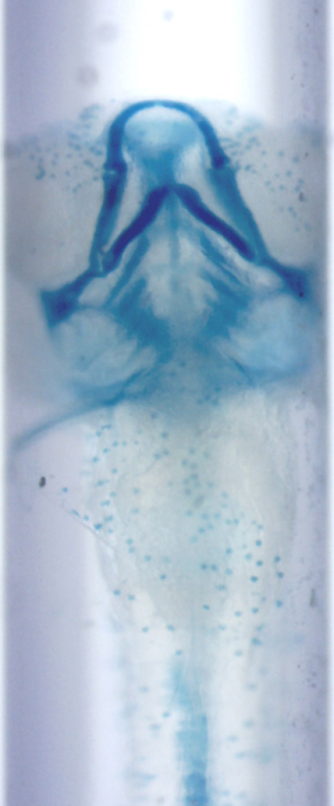
\includegraphics[width=26mm,height=55mm]{figures/research/zf1.png}}
\subfigure[]{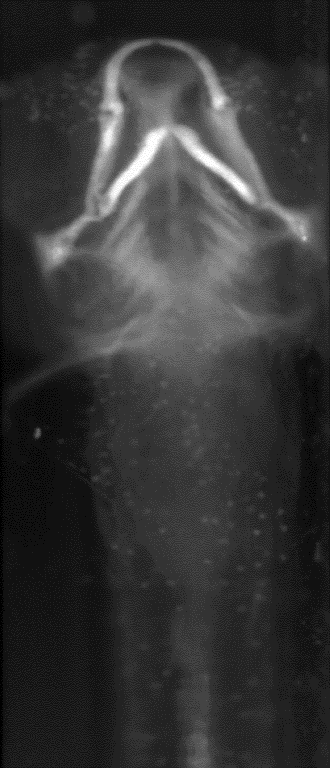
\includegraphics[width=26mm,height=55mm]{figures/research/zf2.png}}
\subfigure[]{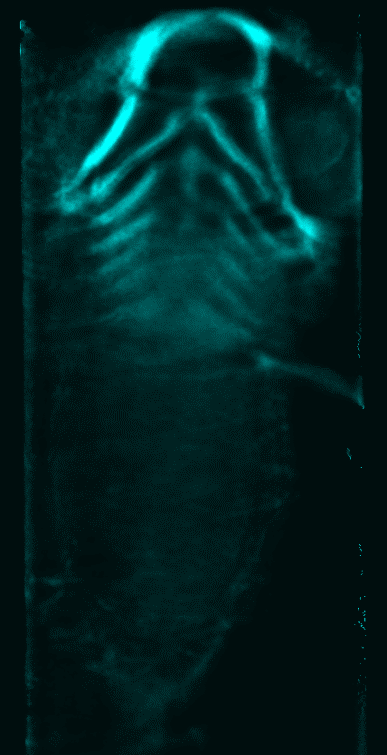
\includegraphics[width=26mm,height=55mm]{figures/research/zf3.png}}
\subfigure[]{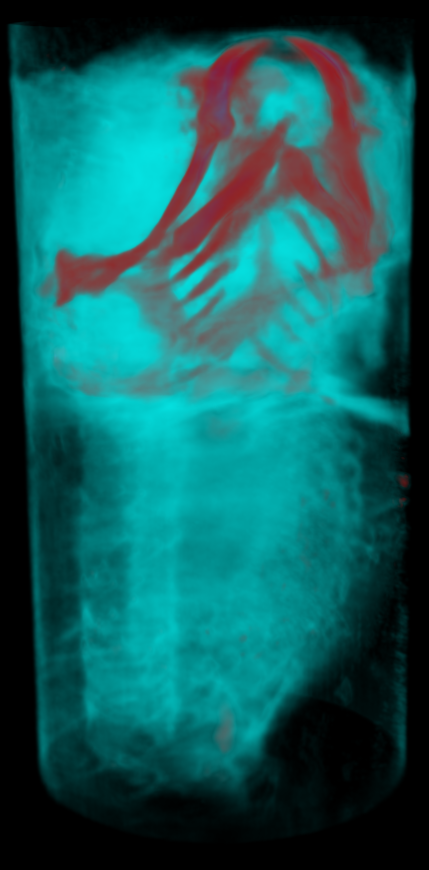
\includegraphics[width=26mm,height=55mm]{figures/research/zf4.png}}
\caption{(a) Recorded projection of a zebrafish embryo. (b) The projection after flat field correction. (c) Reconstructed frontal slice. (d) Volume rendering of the reconstructed image.}
\label{fig::tomography_fish}
\end{figure*}

\begin{figure*}[!htbp]
\centering
\subfigure[]{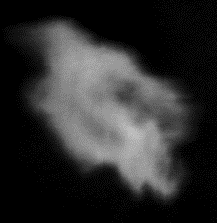
\includegraphics[width=40mm,height=40mm]{figures/research/cell1.png}}
\subfigure[]{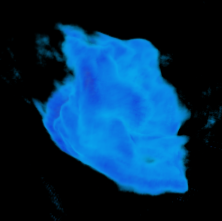
\includegraphics[width=40mm,height=40mm]{figures/research/cell2.png}}
\caption{(a) Projection of a 3D cell culture. (b) Volume rendering of the reconstructed image.}
\label{fig::tomography_cell}
\end{figure*}

%WWW
\item 
\textbf{Image-based Approaches for Drug Tablet Quality Assessment}\\
Ida-Maria Sintorn, Carolina W\"{a}hlby\\
\ppartners{Mark Nicholas, Mats Josefson, AstraZeneca, M\"{o}lndal, Sweden}
\ffunding{Pre-study grant from AIMDay Image, UU Innovation}
\pperiod{1204--1302}
\aabstract{It is known qualitatively that microstructural differences in solid dosage forms (e.g. tablets and inhalation powders) affect the performance of the medication. The microstructural differences are differences in the spatial distribution of active and inactive compounds. The aim of this project is to characterize these microstructural differences in order to determine whether imaging techniques such as CLSM (confocal laser scanning microscopy), wide-field fluorescence microscopy, and TOF-SIMS (Time-Of-Flight Secondary Ion Mass Spectroscopy) can reveal quantifiable differences in structure.  The problem was addressed using a combination of local intensity features and texture measurements (including granulometry, Zernike moments, and Haralick features), and measurements were correlated with tablet characteristics/treatments. Due to a relatively limited dataset, it was difficult to find statistically significant differences. The data was presented to AstraZeneca researchers in January 2013.}

% XXX
\newpage
\item
\label{proj:gigapixel}
\textbf{Tools for Analysis and Visualization of Giga-Pixel Sized  Slide-Scanner Images.}\\
Petter Ranefall, Alexandra Pacureanu, Carolina W\"{a}hlby\\
\ppartners{Mats Nilsson, Thomas Hauling, Marco Mignardi, Jessica Svedlund, Elin Lundin, Department of Biochemistry and Biophysics and SciLifeLab, Stockholm University.}
\ffunding{SciLifeLab}
\pperiod{1308--}
\aabstract{The aim is to create a tool for full resolution image analysis of large images, e.g. slide scanner data, with the possibility of visual examination and interaction at multiple resolutions. The tool is built on a free and open-source framework for visual examination at multiple resolutions with the option to toggle results on or off, such as segmentation masks, classification results, and tissue morphology measurements, using a map view with seamless zooming and panning capabilities, allowing for fast navigation between a full-tissue view and high-resolution sub-cellular observations (Fig. \ref{fig:gigapixel}). The aim is to also have an interface that enables visual/manual selection of regions of interest, target discovery, and understanding of novel spatial relationships within the tissue environment.}

\begin{figure}[!htbp]
\centering
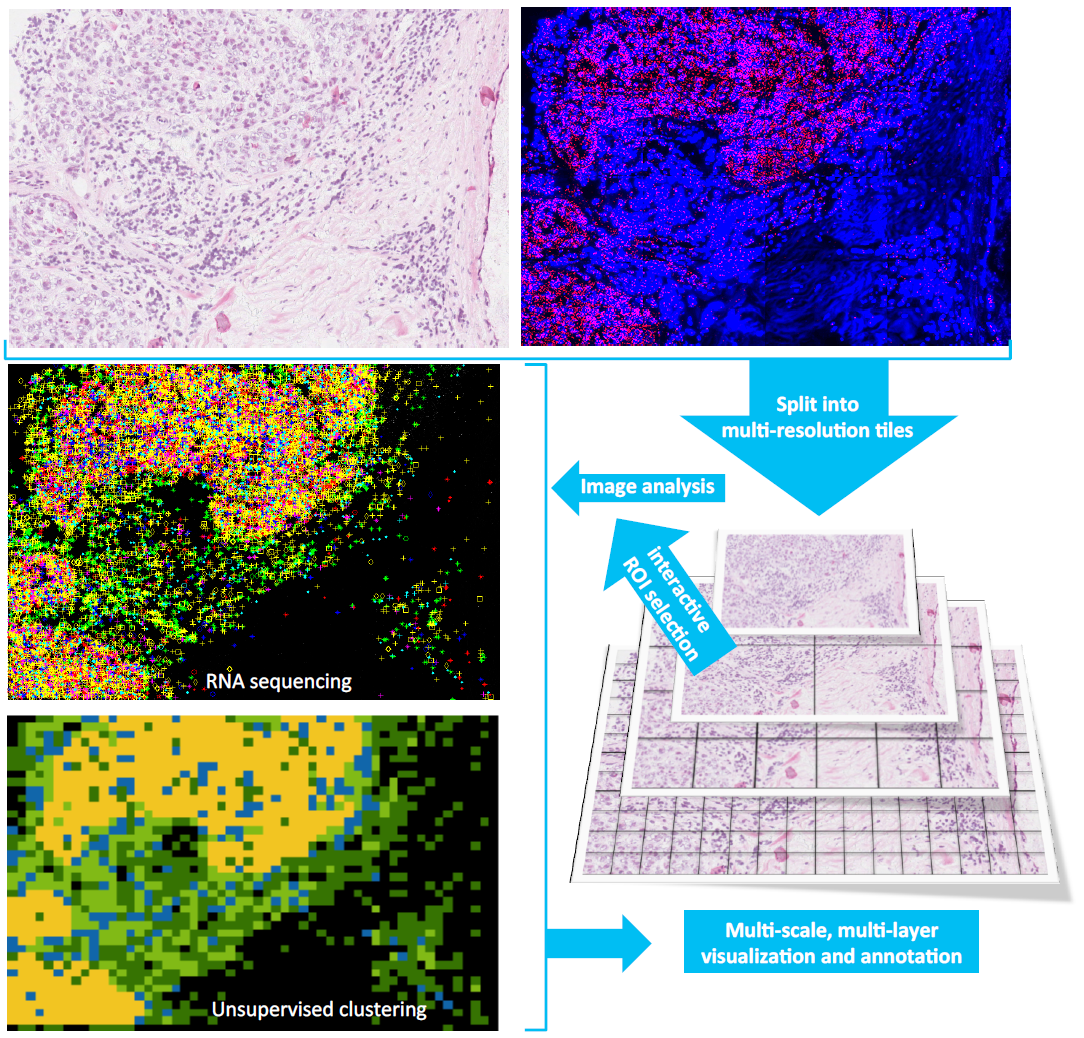
\includegraphics[width=0.8\textwidth]{figures/research/gigapixel.png}
\caption{\label{fig:gigapixel} A description of the workflow.} 
\end{figure}


\clearpage

%-------------------------------------------------------------------------------
%-------------------------------------------------------------------------------
%-------------------------------------------------------------------------------
%-------------------------------------------------------------------------------
%-------------------------------------------------------------------------------

\subsection{3D analysis and visualization}

%AAA

\item 
\label{proj:CMS}
\textbf{Haptics and its Applications to Medicine}\\
Ingrid Carlbom, Stefan Seipel, Pontus Olsson, Fredrik Nysj\"{o}\\
\ppartner{Stefan Johansson (Division of Microsystems Technology, UU and Teknovest AB); Jan-Micha{\'e}l Hirsch, Dept.~of Surgical Sciences, Oral \& Maxillofacial Surgery, UU and Consultant at Dept.~of Plastic- and Maxillofacial Surgery, UU Hospital; Andreas Thor, Dept.~of Surgical Sciences, Oral \& Maxillofacial Surgery, UU Hospital; Andres Rodriguez Lorenzo, Department of Surgical Sciences, Plastic Surgery, UU Hospital; PiezoMotors AB, SenseGraphics AB.}
\ffunding{Dept.~of Surgical Sciences, Oral \& Maxillofacial Surgery, University Hospital}
\pperiod{1301--}
\aabstract{

\textit{Two Degrees-of-Freedom Haptic Gripper with Ultrasonic Piezoelectric Motors} Piezoelectric motors have a high force/mass ratio, which makes them a promising alternative to electromagnetic motors for actuation of haptic interfaces. We have previously developed and evaluated a haptic gripper actuated by a quasi-static piezoelectric motor, operating within the audible range. The evaluation highlighted two main areas for improvement: faster and quieter actuation. During the last year we have designed a new admittance-type haptic gripper (see Figure \ref{fig:haptic1}) with two degrees-of-freedom (DOF), actuated by ultrasonic piezoelectric motors with higher maximum speed and silent operation compared to quasi-static motors. The gripper provides one DOF for the thumb and one DOF for the remaining fingers. All DOFs are direct-drive, involving no mechanical gearing, to minimize backlash and friction. Two custom-made strain-gauge load cells, mounted on the motor axes, measure forces applied by the user.

\begin{figure}[!h]
\centering
\subfigure[]{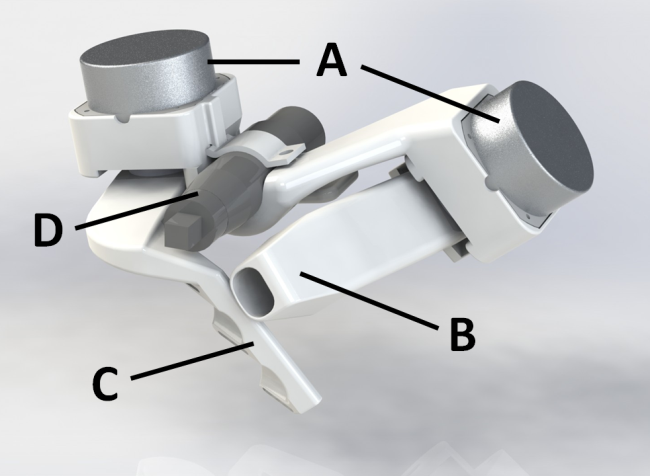
\includegraphics[width=60mm,height=45mm]{figures/research/haptic1.png}}
\subfigure[]{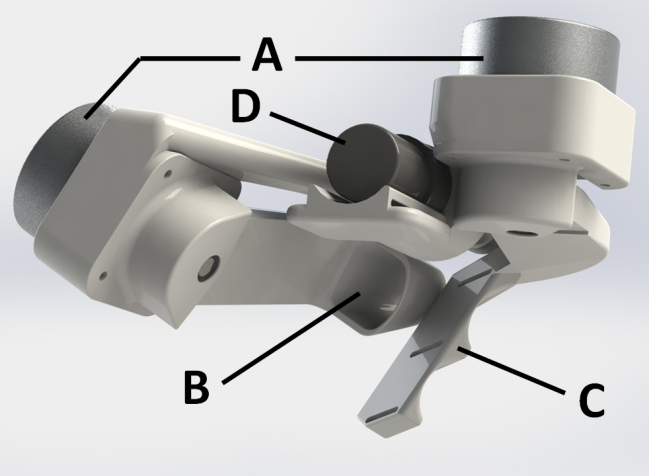
\includegraphics[width=60mm,height=45mm]{figures/research/haptic2.png}}
\caption{\label{fig:haptic1} CAD model of haptic gripper seen from the front (left) and back (right).The ultrasonic piezoelectric motors (A) actuate one DOF for the thumb (B) and one DOF for the remaining fingers (C). The connector (D) may be used to attach the gripper to a commercial six DOF haptic arm, for a total of eight DOF.} 
\end{figure}

\textit{SplineGrip - An Eight Degrees-of-Freedom Flexible Haptic Sculpting Tool} SplineGrip is a flexible haptic sculpting tool that senses the articulation of the hand in two degrees-of-freedom (DOF) that we presented as a SIGGRAPH'13 poster. The tool is mounted on a commercial haptic device that tracks hand pose (position and orientation in six DOF) while simultaneously providing three DOF haptic feedback to the hand. The eight DOF input is mapped to the pose and shape of a virtual representation of a sculpting tool (Figure \ref{fig:haptic2}), offering versatile interaction with a virtual model.

\begin{figure}[!h]
\centering
\subfigure[]{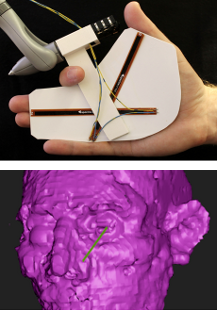
\includegraphics[width=29mm,height=50mm]{figures/research/haptic3.png}}
\subfigure[]{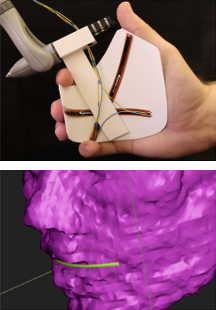
\includegraphics[width=29mm,height=50mm]{figures/research/haptic4.png}}
\subfigure[]{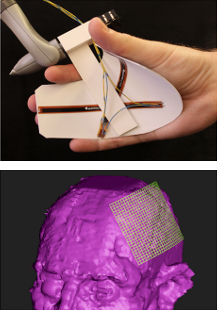
\includegraphics[width=29mm,height=50mm]{figures/research/haptic5.png}}
\subfigure[]{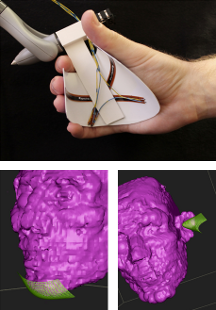
\includegraphics[width=29mm,height=50mm]{figures/research/haptic6.png}}
\caption{\label{fig:haptic2} Example of possible mapping between physical and virtual tool: (a) all fingers straight - the virtual sculpting tool becomes a line segment; (b) middle and ring fingers bent - the curvature of the tool changes; (c) thumb bent - the width of the tool changes; (d) both sensors bent - simultaneous control of curvature and width.} 
\end{figure}
\newpage
\textit{Custom Mandibular Implants} Congenital mandibular bone defects or defects due to tumor resection or trauma often result in substantial functional and aesthetic problems. The use of titanium scaffold implants that may hold bone substitutes for patients that do not require soft tissue transfer has the potential to reduce morbidity, costs, and rehabilitation time.

\begin{figure}[!h]
\centering
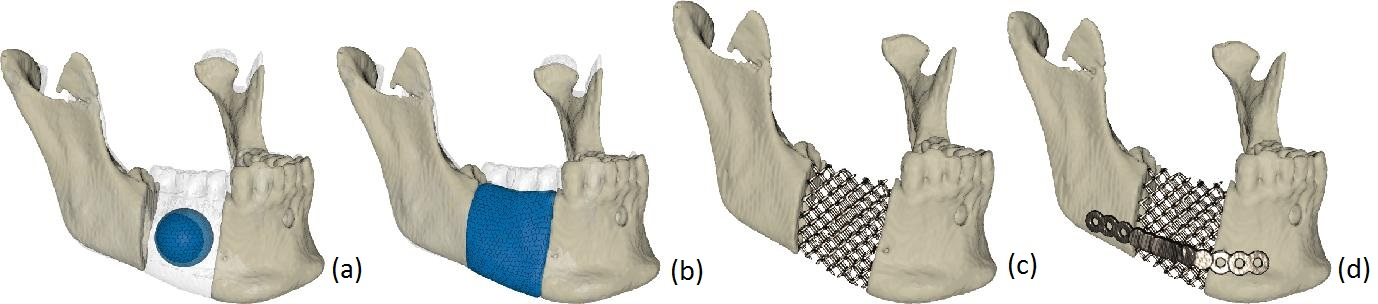
\includegraphics[width=125mm,height=32mm]{figures/research/haptic7.jpg}
\caption{\label{fig:haptic3} Design steps: (a) initialization of the deformable model (blue). Its growth is constrained by a bounding surface (transparent) and the defect surfaces; (b) model growing; (c) fine-tuning and generation of scaffold structure; (d) plate design.} 
\end{figure}

We developed a semi-automatic method based on deformable models and haptics that allows the design and virtual testing of a scaffold implant before production. Using pre-segmented CT-data, a surgeon begins with virtual bone resection, using an interactive cutting tool, to give the defect region good load bearing contact surfaces. Next he/she positions the initial deformable model, which may be a simple sphere, in the defect region and places the bounding surface around the defect (Figure \ref{fig:haptic3}a). The system calculates external forces for the deformable model that expand it towards the defect contact surfaces and the bounding surface until it fills the defect (Figure \ref{fig:haptic3}b). The shape may be adjusted interactively. The surgeon may also refine the implant with the cutting tool and reposition it inside the defect relying on haptic feedback to perfect its fit. The system generates the scaffold structures of the implant (Figure \ref{fig:haptic3}c), and the surgeon may add fixation plates to the structure (Figure \ref{fig:haptic3}d).
}

%----------------------------------------------------------------------------------------------------------------------------------------------

%BBB
\newpage
\item 
\textbf{ProViz -- Interactive Visualization of 3D Protein Images}\\
Lennart Svensson, Ida-Maria Sintorn, Ingela Nystr\"{o}m, Fredrik Nysj\"{o}, Johan Nysj\"{o}, Anders Brun, Gunilla Borgefors\\
\ppartners{Dept.~of Cell and Molecular Biology, Karolinska Institute; SenseGraphics AB}
\ffunding{The Visualization Program by Knowledge Foundation; Vaardal Foundation; Foundation for Strategic Research; VINNOVA; Invest in Sweden Agency}
\pperiod{0807--}
\aabstract{Electron tomography is the only microscopy technique that allows 3-D imaging of biological samples at nano-meter resolution. It thus enables studies of both the dynamics of proteins and individual macromolecular structures in tissue. However, the electron tomography images have a low signal-to-noise ratio, which makes image analysis methods an important tool in interpreting the images. The ProViz project aims at developing visualization and analysis methods in this area.

In general, the project focus 2013 has been on increasing the accessibility of the previously developed methods, by continuing to work on a user-friendly software containing the most important ProViz results. Figure~\ref{fig::proviz} shows how this software can display an electron tomogram, synthetic in this case, and a 3-D fitness landscape showing the matching results for a protein template.

Project highlights during 2013 include a two months research collaboration stay at the Okinawa Institute of Science and Technology, OIST, in Japan and the publishing of a paper at the Iberian Conference on Pattern Recognition and Image Analysis, IbPRIA. During the stay at OIST the software developed in the ProViz project was presented and discussed in depth, with adjustments to the software and improvements to an upcoming manuscript as the result. The research stay was made possible primarily through a JSPS, Japan Society for the Promotion of Science, fellowship. The presented paper concerned a new way of creating registration templates for finding biological structures in electron tomograms.}

\begin{figure*}[!htbp]
\centering
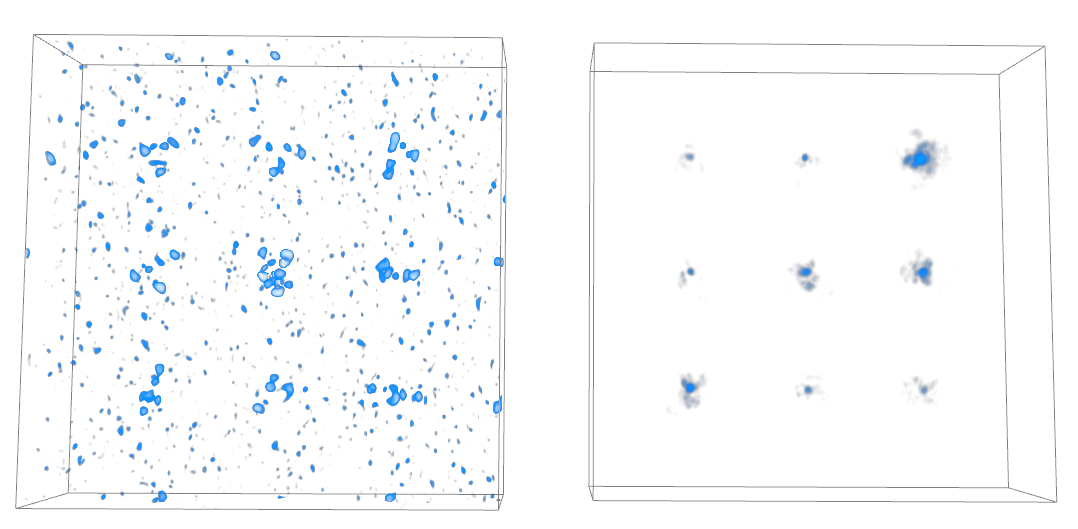
\includegraphics[width=0.9\textwidth]{figures/research/proviz_search_and_score_volumes.PNG}
\caption{For searching an electron tomography image (left) with a molecular template, a standard, but powerful, method is to use a correlation search with a static template. With the ProViz software a 3-D fitness landscape (right), showing the correlation result at different points, can easily be calculated. The electron tomography image to the left is in this case synthetic for evaluation purposes.}
\label{fig::proviz}
\end{figure*}

% CCC
\newpage
\item 
\label{proj:MRI_optimal_lattices}
\textbf{Analysis and Processing of Three-Dimensional Magnetic Resonance Images on Optimal Lattices} \\
Elisabeth Linn\'{e}r, Robin Strand\\
%ppartner{Joel Kullberg, Dept.~of Radiology, Oncology and Radiation Science, UU}
\ffunding{TN-faculty, UU}
\pperiod{1005--}
\aabstract{Three-dimensional images are widely used in, for example, health care. With optimal sampling lattices, the amount of data can be reduced by 30\% without affecting the image quality. In this project, methods for image acquisition, analysis and visualization using optimal sampling lattices are studied and developed, with special focus on magnetic resonance imaging. The intention is that this project will lead to faster and better processing of images with less demands on data storage capacity.

During 2013, the focus has been on distance transforms. A paper describing a graph-based implementation of the anti-aliased Euclidean distance transform was submitted for publication.}

% DDD

\item 
\label{proj:MRI_registration}
\textbf{Registration of Medical Volume Images}\\
Robin Strand, Filip Malmberg\\
\ppartner{Joel Kullberg, H{\aa}kan Ahlstr\"{o}m, Dept.~of Radiology, Oncology and Radiation Science, UU}
\ffunding{Faculty of Medicine, UU}
\pperiod{1208--}
\aabstract{In this project, we mainly process magnetic resonance tomography (MR) images. MR images are very useful in clinical use and in medical research, e.g., for analyzing the composition of the human body. At the division of Radiology, UU, a huge amount of MR data, including whole body MR images is acquired for research on the connection between the composition of the human body and disease.

To compare volume images voxel by voxel, we develop image registration methods. For example, large scale analysis is enabled by image registration methods that utilizes, for example, segmented tissue (see, e.g., Project~\ref{project:medical_segmentation}) and anatomical landmarks. Another example is interactive image registration where a user can fine-tune the segmentation result by a user interface, see Figure~\ref{fig:interactive_image_registration}.}

\begin{figure}[!htbp]
\centering
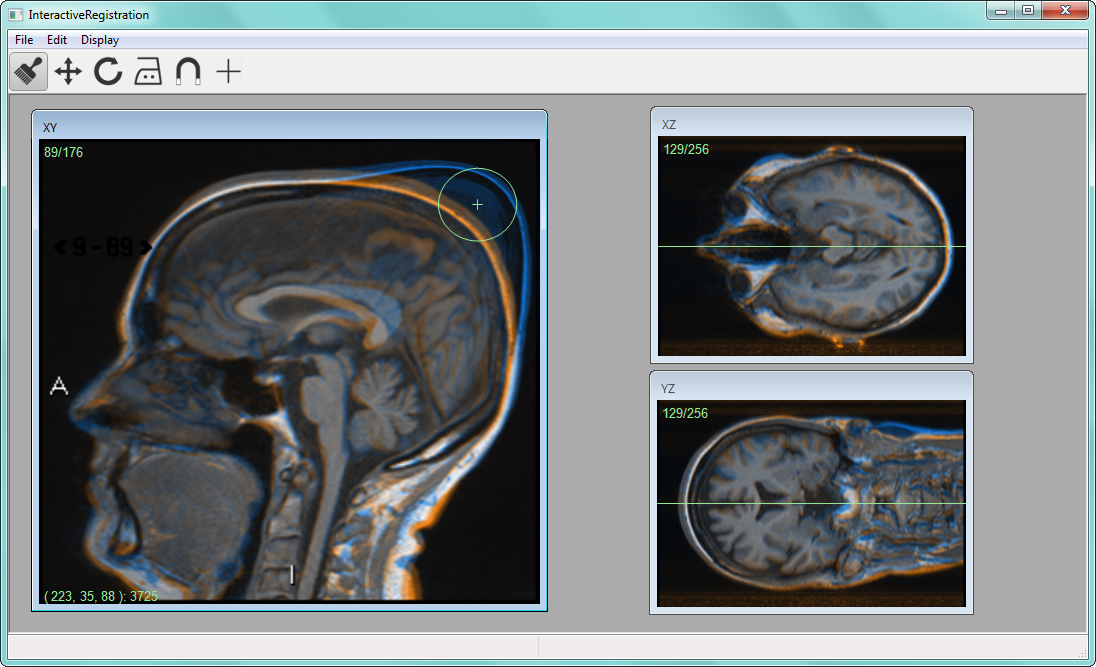
\includegraphics[width=0.65\textwidth]{figures/research/interactive_image_registration.png}
\caption{\label{fig:interactive_image_registration} A screen-shot of the user interface of our software for interactive deformable registration. The target image and the transformed source image are displayed using a colored overlay in three orthogonal views. The user can deform the source image by clicking and dragging in any of the views, as shown in the screen-shot.}
\end{figure}

% EEE
\newpage
\item 
\label{project:medical_segmentation}
\textbf{Interactive Segmentation and Analysis of Medical Images}\\
Filip Malmberg, Robin Strand, Ingela Nystr{\"o}m, Ewert Bengtsson\\
\ppartners{Joel Kullberg, H{\aa}kan Ahlstr\"{o}m, Dept.~of Radiology, Oncology and Radiation Science, UU}
\ffunding{TN-faculty, UU}
\period{1106--}\\
\aabstract{Three-dimensional imaging technique such as computed tomography (CT) and magnetic resonance imaging (MRI ) are now routinely used in medicine. This has lead to an ever increasing flow of high-resolution, high-dimensional, image data that needs to be qualitatively and quantitatively analyzed. Typically, this analysis requires accurate segmentation of the image. 

At CBA, we have been developing powerful new methods for interactive image segmentation (see Project~\ref{project:interactive_segmentation}). In this project, We seek to employ these methods for segmentation of medical images, in collaboration with the Dept.~of Radiology, Oncology and Radiation Science at the UU Hospital. In 2013 a software for interactive segmentation, called \emph{Smartpaint}, was made publicly available (Fig. \ref{fig:smartpaint}). The software can be downloaded from \url{http://www.cb.uu.se/~filip/SmartPaint/}.}

\begin{figure}[!h]
\centering
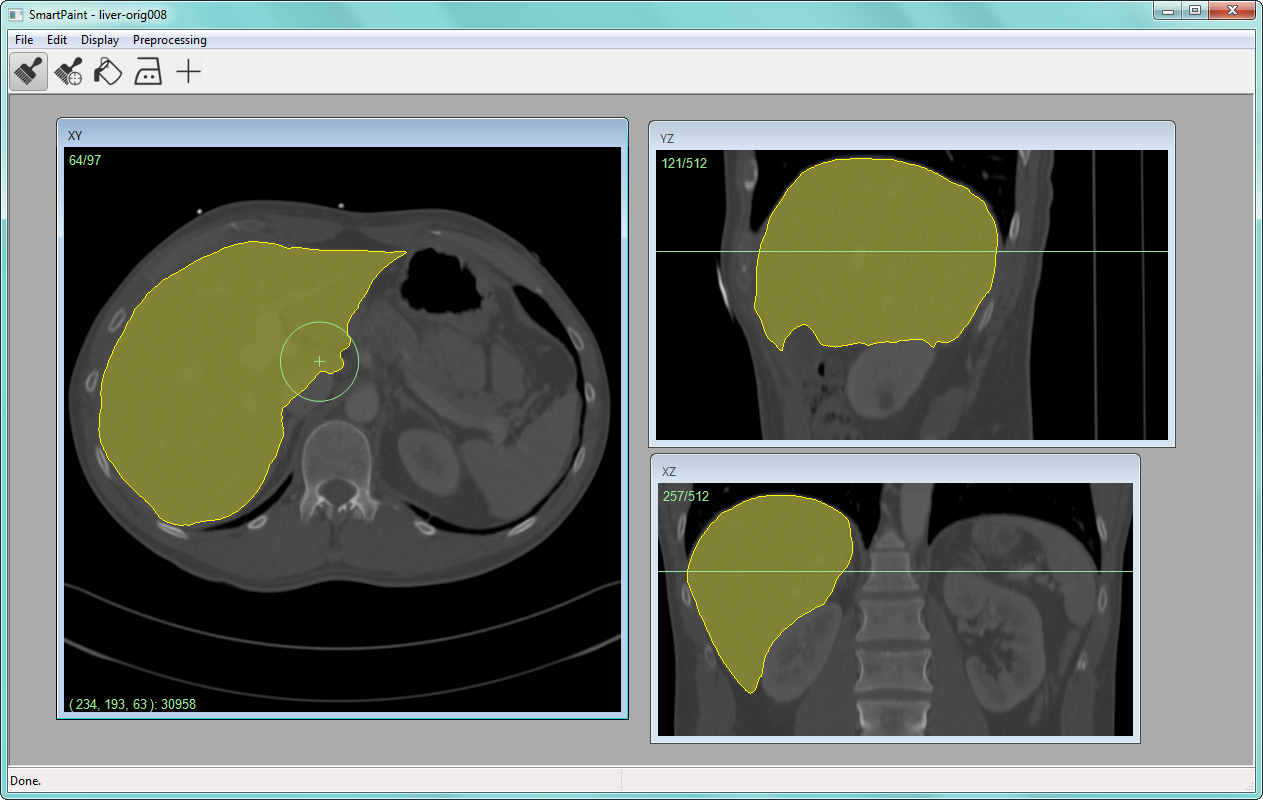
\includegraphics[width=0.6\textwidth]{figures/research/SP_Screenshot.png}
\caption{\label{fig:smartpaint} Screenshot from the \emph{Smartpaint} software for interactive segmentation of volume images, developed at CBA. A radiologist segments the prostate in a MR image by interactively ``painting'' the segmentation using a brush tool.} 
\end{figure}

% FFF

\item
\label{project:orbit_segmentation}
\textbf{Orbit Segmentation for Cranio-Maxillofacial Surgery Planning}\\
Filip Malmberg, Ewert Bengtsson, Ingela Nystr{\"o}m, Johan Nysj\"{o}\\
\ppartners{Jan Michael Hirsch, Andreas Thor, Johanna Nilsson, Dept.~of Surgical Sciences, UU Hospital; Roman Khonsari, Pitie Salpetriere Hospital, Paris, France; Jonathan Britto, Great Ormond Street Hospital, London, United Kingdom}
\ffunding{TN-faculty, UU; NovaMedTech}
\pperiod{0912--}
\aabstract{A central problem in cranio-maxillofacial (CMF) surgery is to restore the normal anatomy of the skeleton after defects, i.e., malformations, tumors and trauma to the face. This is particularly difficult when a fracture causes vital anatomical structures such as the bone segments to be displaced significantly from their proper position, when bone segments are missing, or when a bone segment is located in such a position that any attempt to restore it into its original position poses considerable risk for causing further damage to vital anatomical structures such as the eye or the central nervous system. There is ample evidence that careful pre-operative planning can significantly improve the precision and predictability and reduce morbidity of the craniofacial reconstruction. In addition, time in the operating room can be reduced. An important component in surgery planning is to be able to accurately measure the extent of certain anatomical structures. Of particular interest in CMF surgery are the shape and volume of the orbits (eye sockets) comparing the left side with the right side. These properties can be measured in CT images of the skull, but this requires accurate segmentation of the orbits. Today, segmentation is usually performed by manual tracing of the orbit in a large number of slices of the CT image. This task is very time-consuming, and sensitive to operator errors. Semi-automatic segmentation methods could reduce the required operator time significantly. In this project, we are developing a prototype of a semi-automatic system for segmenting the orbit in CT images. The segmentation system is based on WISH, a software package for interactive visualization and segmentation that has been developed at CBA since 2003. WISH has been released under an open-source license and is available for download at \url{http://www.cb.uu.se/research/haptics}.

In 2011, a paper about the orbit segmentation system was presented at the International Visual Information Conference (IVIC) in Malaysia. We also started investigating other applications for the system, e.g., volumetric measurements of the airway space in cone beam CT images and volumetric measurements of the maxillary sinuses in CT images.

\begin{figure*}[!htbp]
\centering
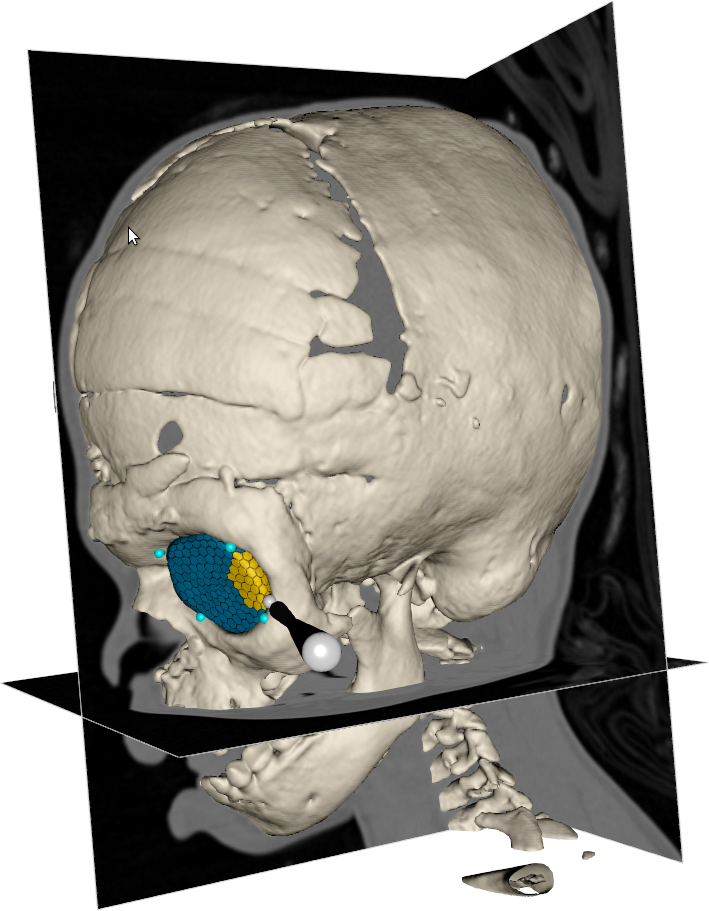
\includegraphics[width=75mm,height=90mm]{figures/research/orbit_project_figure1.png}
\caption{Haptic-aided semi-automatic segmentation of the left orbit (eye-socket) in a post-operative CT scan of a patient suffering from Crouzon syndrom, a congenital disorder that makes the orbits smaller and more shallow than normal.}
\label{fig:orbit1}
\end{figure*}

During 2013, we have been collaborating with people from the Craniofacial Centre at Great Ormond Street Hospital, London, United Kingdom, in a project that aims to analyse the size and shape of the orbits in pre- and post-operative CT images of patients with congenital disorders. The semi-automatic segmentation system has been used to segment the orbits in these datasets (Fig. \ref{fig:orbit1}), and we have developed automatic tools for performing size and shape analysis of the segmented orbits (Fig. \ref{fig:orbit2}). Several abstracts about the ongoing work has been presented at medical conferences. Next, we plan to summarize the collected data and extend the abstracts to journal publications. In addition, we have performed two smaller orbit segmentation studies together with people from the UU hospital, resulting in one presented abstract at Tandl\"{a}karnas Riksst\"{a}mma. In collaboration with Roman Khonsari at Pitie Salpetriere Hospital, Paris, France, we also published a paper on shape and volume measurements on intentionally deformed skulls in American Journal of Physical Anthropology.}

\begin{figure*}[!htbp]
\centering
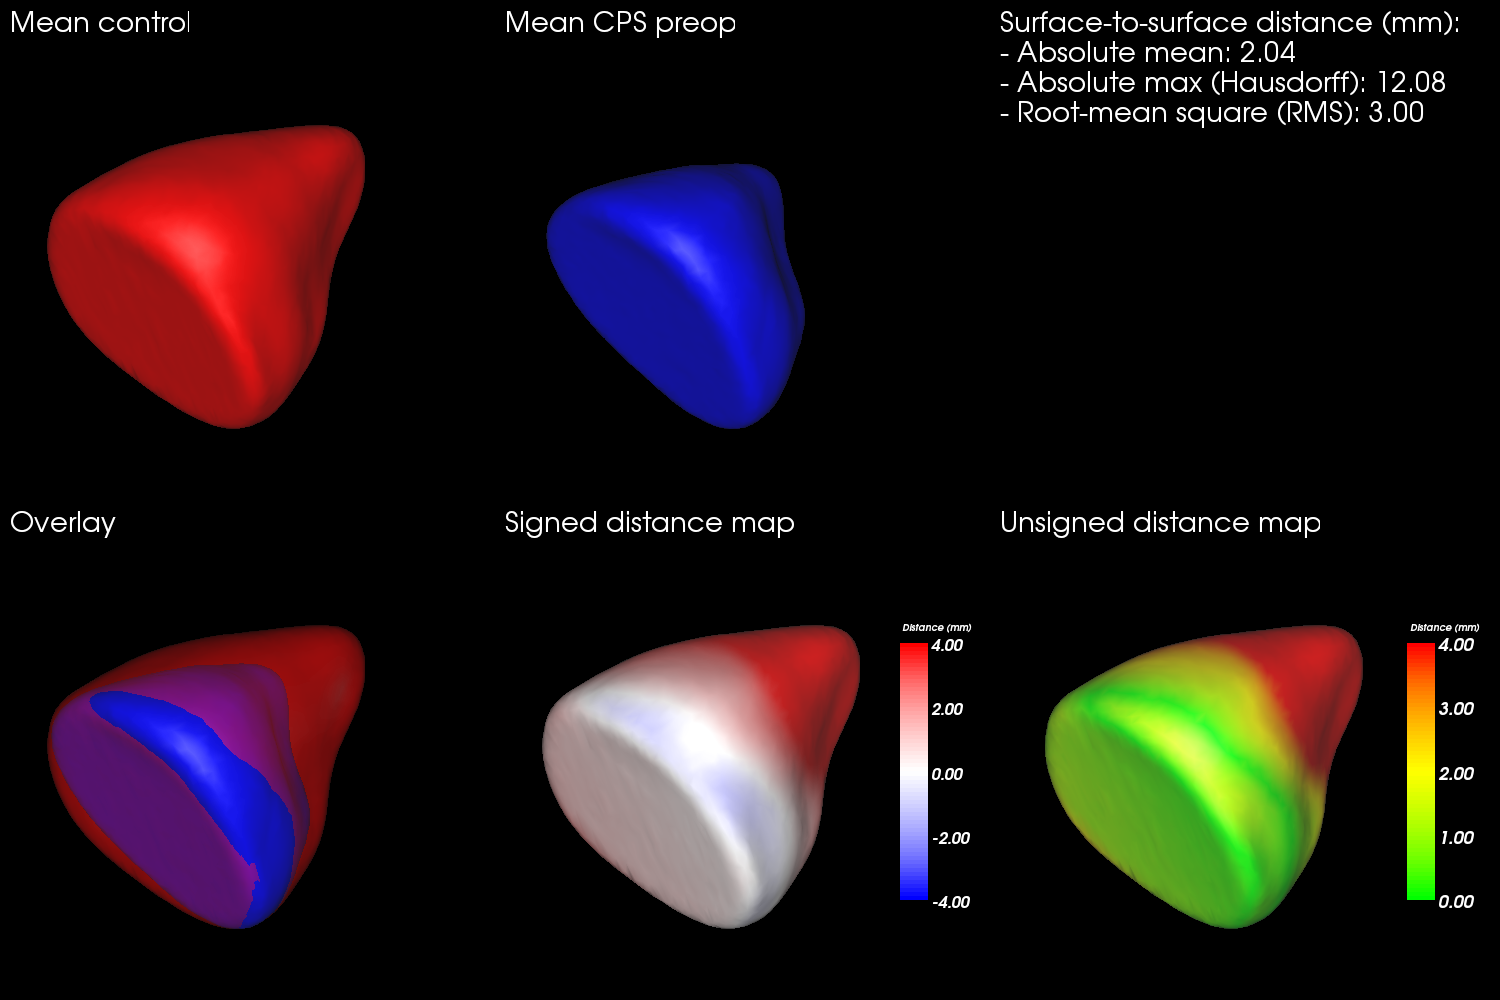
\includegraphics[width=0.9\textwidth]{figures/research/orbit_project_figure2.png}
\caption{Registration-based comparison of automatically constructed mean size and shape models of the orbit. In this case, a mean control model of normal orbits is compared against a mean model of pre-operative orbits from patients suffering from congenital disorder called Crouzon-Pfeiffer syndrome (CPS). The semi-transparent surface overlays and color-coded distance maps shows that CPS orbits tend to be smaller and more shallow than normal orbits.}
\label{fig:orbit2}
\end{figure*}

% GGG

\item 
\label{project:wrist_angle_measurements}
\textbf{Precise 3D Angle Measurements in CT Wrist Images}\\
Filip Malmberg, Johan Nysj{\"o}, Ingela Nystr{\"o}m, Ida-Maria Sintorn\\
\ppartners{Albert Christersson, Dept.~of Orthopedics, UU Hospital}
\ffunding{TN-faculty, UU}
\pperiod{1111--}
\aabstract{To be able to decide the correct treatment of a fracture, for example, whether a fracture needs to be operated on or not, orthopedic surgeons need to assess the details about the fracture. One of the most important factors is the fracture displacement, particularly the angulation of the fracture. When a fracture is located close to a joint, for example, in the wrist, which is the most common location for fractures in the human being, the angulation of the joint line in relation to the long axis of the long bone needs to be measured (Fig. \ref{fig:wrist}a). Since the surface of the joint line in the wrist is highly irregular, and since it is difficult to take X-rays of the wrist in exactly the same projections from time to time, conventional X-ray is not an optimal method for this purpose. In most clinical cases, conventional 2D angle measurements in X-ray images are satisfactory for making correct decisions about treatment, but when comparing two different methods of treatment, for instance, two different operation techniques, the accuracy and precision of the angle measurements need to be higher.

In this project, we are developing a system for performing precise angle measurements in 3D computed tomography (CT) images of the wrist (Fig. \ref{fig:wrist}b). Our proposed system is semi-automatic; the user is required to guide the system by indicating the approximate position and orientation of various parts of the radius bone. This information is subsequently used as input to an automatic algorithm that makes precise angle measurements. A RANSAC-based method for estimating the long axis of the radius bone was presented at the International Conference on Computer Vision and Graphics (ICCVG' 2012). During 2013, we developed a registration-based method for measuring the orientation of the joint surface of the radius. This method was combined with the previously developed axis estimation method and presented at ICIAP 2013. Currently, we are performing a more extensive case study (involving 40 CT scan sequences of fractures wrists) to further evaluate the performance of the 3D angle measurement method and compare it with the conventional 2D X-ray measurement method.}

\begin{figure}[!htbp]
\centering
\begin{tabular}{c}
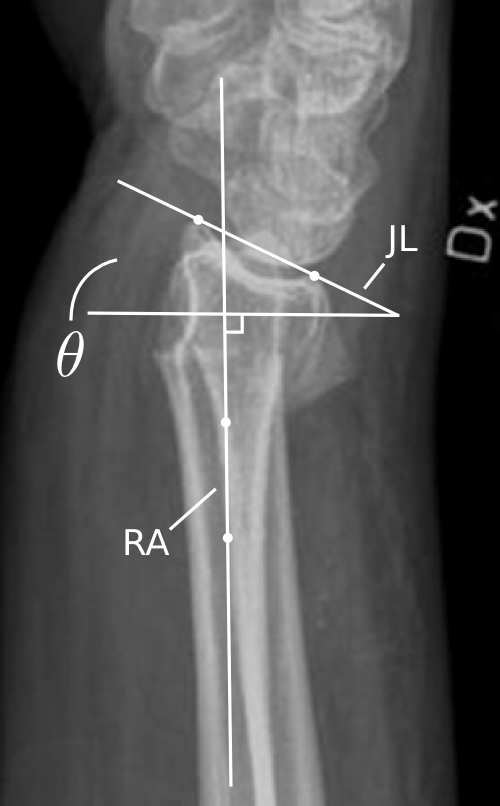
\includegraphics[width=0.4\textwidth]{figures/research/wrist_project_figure1a.png}
\vspace*{2mm}
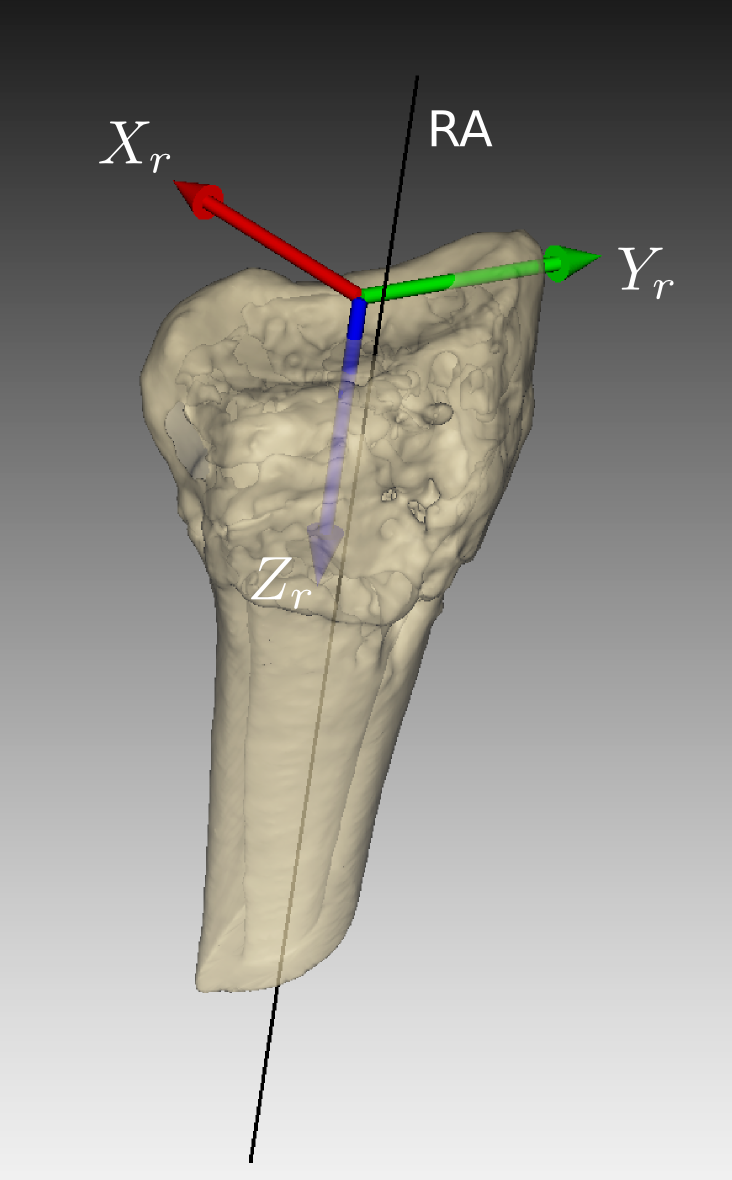
\includegraphics[width=0.4\textwidth]{figures/research/wrist_project_figure1b.png}
\end{tabular}
\caption{\label{fig:wrist} (a) The dorsal angle, $\theta$, measured in 2D on a lateral X-ray image of the radius bone in the wrist. $\theta$ is defined as the angle between the joint line JL and a line that is orthogonal to the long axis RA of the radius. (b) A 3D rendering of the radius bone and the reference axes we identify to measure the dorsal angle in 3D.}
\end{figure}

% HHH

\item \textbf{Efficient Algorithms for Computer Graphics}\\
Ewert Bengtsson, Anders Hast \\
\ppartner{Tony Barrera, Uppsala}
\ffunding{TN-faculty, UU}
\pperiod{9911--}
\aabstract{Computer graphics is increasingly being used to create realistic images of 3D objects for applications in entertainment, (animated films, games), commerce (showing 3D images of products on the web), industrial design and medicine. For the images to look realistic high quality shading and surface texture and topology rendering is necessary. A proper understanding of the mathematics behind the algorithms can make a big difference in rendering quality as well as speed. We have in this project over the years re-examined several of the established algorithms and found new mathematical ways of simplifying the expressions and increasing the implementation speeds without sacrificing image quality. We have also invented a number of completely new algorithms. The project is carried out in close collaboration with Tony Barrera, an autodidact mathematician. It has been running since 1999 and resulted in more than 25 international publications and a PhD thesis.

During 2013 a poster was accepted for the ACM Computing Frontiers conference entitled: "An Algorithm for Parallel Calculation of Trigonometric and Exponential Functions".}

% III

\item \textbf{Ubiquitous Visualization in the Built Environment}\\
Stefan Seipel, Fei Liu\\
\ffunding{University of G\"{a}vle; TN-faculty, UU}
\pperiod{110801--}%20150801}
\aabstract{This research project in ubiquitous visualization deals with mobile visualization of spatial data in indoor and outdoor environments. Several key problems for robust mobile visualization are addressed such as spatial tracking and calibration, image based 2D and 3D registration and efficient graphical representations in mobile user interfaces. During 2013 we have devised a fasade region detection method by analyzing image profiles for repetitive patterns in street view images. These profiles are generated by scanning the hue channel of images along lines constructed with edge line segments and vanishing points. The work has been compiled into a paper titled "Detection of Fasade Regions in Street View Images from Split-and-Merge of Perspective Patches" and submitted to the International Conference on Computing and Computer Vision 2014. Meanwhile, we have also been exploring various image features to describe the detected fasade regions in order to identify which building is presented in a specific image.}

\clearpage

%-------------------------------------------------------------------------------
%-------------------------------------------------------------------------------
%-------------------------------------------------------------------------------
%-------------------------------------------------------------------------------
%-------------------------------------------------------------------------------

\subsection{Theory: discrete geometry, mathematical morphology and volume processing}

\item
\label{project:interactive_segmentation}
\textbf{Improved Methods for Interactive Graph-Based Segmentation}\\
Filip Malmberg, Robin Strand, Ingela Nystr\"{o}m, Ewert Bengtsson\\
\ffunding{TN-faculty, UU}
\period{0901--}\\
\aabstract{Image segmentation, the process of identifying and separating relevant objects and structures in an image, is a fundamental problem in image analysis. Accurate segmentation of objects of interest is often required before further processing and analysis can be performed. Despite years of active research, fully automatic segmentation of arbitrary images remains an unsolved problem. 

\emph{Interactive} segmentation methods use human expert knowledge as additional input, thereby making the segmentation problem more tractable. A successful semi-automatic method minimizes the required user interaction time, while maintaining tight user control to guarantee the correctness of the result. The input from the user is typically given in one of two forms:

\begin{description}
\item \textit{Boundary constraints} The user is asked to provide pieces of the desired segmentation boundary.
\item \textit{Regional constraints} The user is asked to provide a partial labeling of the image elements (e.g., marking a small number of image elements as ``object'' or ``background'').
\end{description}

Interactive segmentation is often phrased as an optimization problem, i.e., a solution is sought that optimizes some  criterion on segmentation ``goodness'' while satisfyng the constrains provided by the user. In this project, we develop new methods for interactive segmentation, using a combinatorial approach. In 2013, results from this project were presented at the International Symposium on Mathematical Morphology (ISMM) is Uppsala.} 

% BBB

\item
\label{proj:stochwatershed}
\textbf{The Stochastic Watershed}\\
Bettina Selig, Cris Luengo, Ida-Maria Sintorn, Filip Malmberg\\
\ffunding{S-faculty, SLU}
\pperiod{1102--}
\aabstract{The stochastic watershed is a method recently presented that builds on the classical seeded watershed algorithm. It creates a probability density function for edges in the image by repeated applications of the seeded watershed with random seeds. We have found that adding noise to the input image before every application of the seeded watershed greatly improves the properties of the output. These results were published this year in Pattern Recognition Letters. This year we have developed an efficient algorithm that computes the result one
would obtain after an infinite number of repetitions of the seeded watershed, and have been working towards a method to combine this algorithm with the improvements presented in our previous paper.}

%CCC

\item 
\textbf{Adaptive Mathematical Morphology}\\
Vladimir \' Curi\' c, Cris Luengo, Gunilla Borgefors\\
\ppartner{Jes\' us Angulo, Centre for Mathematical Morphology, Ecole des Mines de Paris - MINES ParisTech, Fontainebleau, France; 
Anders Landstr\" om, Matthew Thurley, Lule\aa\, University of Technology, Lule\aa ;
S\' ebastien Lef\`{e}vre, University of South Brittany, Vannes, France;
Santiago Velasco-Forero, National University of Singapore, Republic of Singapore.}
\ffunding{Graduate School in Mathematics and Computing (FMB)}
\pperiod{1101--}
\aabstract{The construction of adaptive structuring elements that adjust their shape and size to the local structures in the image has recently been a popular topic in mathematical morphology. Despite that several methods for the construction of spatially adaptive structuring elements have been proposed, it is still an open problem, both from a theoretical and implementation point of view.

We have proposed salience adaptive structuring elements that modify their shape and size according to the saliency of the edges in the image. We have examined topological properties of salience adaptive structuring elements and investigated their applicability to image filtering. This work has been published in IEEE Journal of Selected Topics in Signal Processing. We have also proposed structuring elements with predefined shape and adaptive size based on similar type of the salience map as it was used for the construction of the salience adaptive structuring elements. Furthermore, we extended this work to salience-based parabolic structuring functions, which was presented at the International Symposium on Mathematical Morphology (ISMM'2013). More recently, we perform a comparative study of a few most important methods for constructing adaptive structuring elements as well theoretical advances how to properly define respective morphological operators. This work is currently under review.

We intend to further investigate theoretical properties of adaptive morphological operators as well as apply such operators to the task of image regularization. An extension of adaptive morphological operators towards multi-valued images and their definitions for sparse image representations are of interest in future studies.}

%DDD

\item 
\label{proj:DT}
\textbf{Digital Distance Functions and Distance Transforms} \\
Robin Strand, Gunilla Borgefors \\
\ppartner{Benedek Nagy, Dept.~of Computer Science, Faculty of Informatics, University of Debrecen, Hungary; Nicols Normand, IRCCyN, University of Nantes, France}
\ffunding{TN-faculty, UU; S-faculty, SLU}
\pperiod{9309--}
\aabstract{The distance between any two grid points in a grid is defined by a distance function. In this project, weighted distances have been considered for many years. A generalization of the weighted distances is obtained by using both weights and a \textit{neighborhood sequence} to define the distance function. The neighborhood sequence allows the size of the neighborhood to vary along the paths. 

In 2013, papers on 
\begin{itemize}
\item the link between digital distance functions and integer sequences, through Beatty sequences and the Lambek-Moser inverse,
\item weight sequence distance functions, where weighted neighborhood sequences of infinte length are allowed, and
\item efficient computation of digital distance transforms, 
\end{itemize}
have been published in Computer Vision and Image Understanding and proceedings of DGCI and ISMM.}

% EEE

\item 
\label{proj:MBD}
\textbf{The Minimum Barrier Distance}\\
Robin Strand, Filip Malmberg\\
\ppartner{Punam K. Saha, Dept.~of Electrical and Computer Engineering and the Dept.~of Radiology, University of Iowa, IA, USA; Krzysztof C. Ciesielski, Dept.~of Mathematics, West Virginia University, Morgantown, WV, USA; Dept.~of Radiology, MIPG, University of Pennsylvania, PA, USA}
\ffunding{TN-faculty, UU}
\pperiod{1103--}
\aabstract{In this project, we introduce a distance function on a fuzzy subset that gives the minimum barrier that has to be passed to go from one point to another. Theoretical properties as well as efficient computational solutions for minimum barrier distance have been developed. An initial application of minimum barrier distance in image segmentation is presented. The experiments show that the minimum barrier distance is robust to noise and blur, and also seed point position, since it captures the total change in membership values across an interface instead of gradient as a measure of slope that is sensitive to noise and blur.

A paper on the theoretical foundation of the minimum barrier distance was published in Computer Vision and Image Understanding. Our work in this project during 2013 has been focused on finding efficient, and exact, algorithms for computing the minimum barrier distance.}

%FFF

\item
\label{proj:set_dist}
\textbf{Set Distances and their Application in Image Analysis}\\
Vladimir \' Curi\' c, Gunilla Borgefors\\
\ppartner{Joakim Lindblad, Nata\v sa Sladoje, Faculty of Technical Sciences, University of Novi Sad, Serbia}
\ffunding{Graduate School in Mathematics and Computing (FMB)}
\pperiod{0908--}
\aabstract{Methods for measuring distances between sets, which is a measure of how similar the sets are, can be useful for solving various image analysis related problems, such as registration, image retrieval and segmentation evaluation. Depending on how the distance measure is defined, it exhibits different properties, such as metricity, monotonicity, continuity, sensitivity to noise, complexity and speed of computation. It is therefore of interest to study and further develop different set distance measures, to be able to select appropriate distances for the different applications. In this project, we evaluate existing and develop new set distances which are useful in image registration related problems.
We have proposed a new set distance between crisp sets of points and evaluated its usefulness for rigid body registration of binary images as well as its applicability for the real task of multi-modal 2D-3D registration of 2D histological sections of bone implant with corresponding 3D synchrotron radiation micro computed tomography (SR\textmu CT) bone implant volumes. In addition, it has been shown that this set distance has good performances when applicable to the task of recognition of handwritten characters. This work has been accepted for publication to Pattern Analysis and Applications.

We extended our study to fuzzy objects and proposed four novel point-to-set distances defined for fuzzy or gray-level image data, two based on integration of alpha cuts and two based on the fuzzy distance transform. We further used these point-to-set distances to define distances between fuzzy sets. Theoretical study and performance evaluation of the proposed distances confirm their excellent behaviour in template matching and object classification. New distance measures enable to include and consider both spatial and intensity information, which makes them applicable to texture matching problems as well. The results of this study have been published in IEEE Transactions on Image Processing.}

% GGG

\item
\textbf{Direct Curvature Calculation of Surfaces in 3D Volumes }\\
Erik Wernersson, Cris Luengo, Anders Brun, Gunilla Borgefors \\
\ffunding{S-faculty, SLU}
\pperiod{1009 --}
\aabstract{Curvature is known to be a useful local descriptor of 2D surfaces, embedded in 3D space. Not only for parametric surfaces but
also estimated from objects in digital images with applications ranging from visualisation to segmentation. 

Within this project, we have studied curvature calculated from the structure tensor, in contrast to the most common methods which derive
curvature directly from image differentials. This opens up for new kind of processing, and especially averaging, which we hope will be of
interest for the analysis of wood fibres in \textmu CT images of paper and composite materials.}

\clearpage

%----------------------------------------------------------------------------------------------------------------------------------------------
%----------------------------------------------------------------------------------------------------------------------------------------------
%----------------------------------------------------------------------------------------------------------------------------------------------
%----------------------------------------------------------------------------------------------------------------------------------------------
%----------------------------------------------------------------------------------------------------------------------------------------------

\subsection{Other projects}

% AAA

\item \textbf{Optical Character Recognition of Handwritten Texts}\\
Anders Brun, Ewert Bengtsson, Fredrik Wahlberg, Tomas Wilkinson, Kalyan Ram\\
\ppartners{Lasse M{\aa}rtensson, Dept.~of Scandinavian Languages, UU; Mats Dahll\"{o}f, Dept.~of Linguistics and Philology, UU}
\ffunding{Faculty of Languages and Humanities, UU}
\pperiod{1008--}
\aabstract{Optical character recognition (OCR) is still, after nearly 100 years of research, an active area of research. Currently one of the frontiers is the recognition of handwritten text (HTR), in particular from historical documents, see Figure~\ref{fig:OCR}. This year, two PhD students were recruited. Bojana Simsic was hired to do part-time work on marketing. The project participated in the book fair Bokm\"{a}ssan in Gothenburg and was featured several times in articles and on national TV. In late 2013, the project started to collaborate with The Swedish Museum of Natural History, to help out with digitization of herbarium sheets.}

\begin{figure}[!htbp]
\centering
\includegraphics[width=0.6\textwidth]{figures/research/cba_ar.png}
\caption{\label{fig:OCR} Detail of spread 198 from "Summula de ministris et sacramentis ecclesiasticis" written by Laurentius of Vaksala in the 14th century. 
} 
\end{figure}

%BBB

\item
\label{proj:geomemories}
\textbf{GeoMemories}\\
Anders Hast\\
\ppartners{Andrea Marchetti, Salvatore Minutoli, Alessandro Prosperi, Alessandro Lugari, Maurizio Tesconi, Beatrice Rapisarda, Matteo Abrate, Clara Bacciu, Davide Gazz\'e, Sergio Bianchi, Istituto di Informatica e Telematica (IIT), Pisa, Italy}
\aabstract{The GeoMemories project is aimed at making publicly available, through  web access, heritage preserved in the archives of Aerofototeca  Nazionale in Rome, which contains photographs covering the Italian  territory from the end of 1800 till modern days. The web application  is based on google earth but oriented towards the management of the  temporal variable, so that geospatial changes can be monitored over  time. The historical aerial photos need to be digitized, illumination  corrected, orthorectified, georeferenced and finally stitched together.
Anders Hast spent one year (2011) at IIT, CNR in Pisa Italy as an  ERCIM fellow working with image processing and computer vision aspects  in the project. Since returning to UU in January he is  a research associate at IIT, CNR and continues working with the project.

During 2013 three papers were published, whereof two journal papers  and one conference paper. One of the journal papers describes the  GeoMemories application and the image pipeline being used, and was  accepted in a Special Issue "Geospatial Monitoring and Modelling of  Environmental Change" of the ISPRS International Journal of  Geo-Information. The title is "Geomemories - A Platform for  Visualizing Historical, Environmental and Geospatial Changes of the  Italian Landscape". The Figure \ref{fig:pisa} is taken from that paper and shows how the application can be used to monitor environmental changes. About  400 meters of the shore line outside Pisa has disappeared since 1943,  and even more since 1765 (cadastral map).}

\begin{figure}[!htbp]
\centering
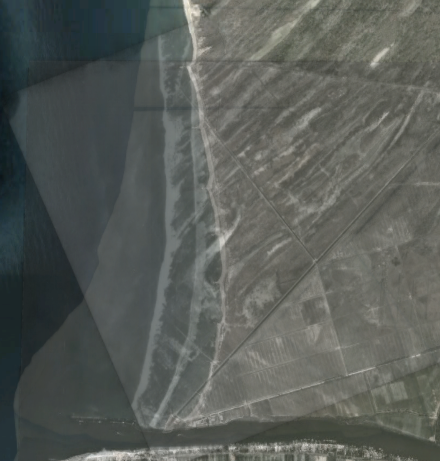
\includegraphics[width=0.6\textwidth]{figures/research/foce_all.png}
\caption{\label{fig:pisa} This blended photo makes it possible to study how the costal shore line outside Pisa has changed and moved in time and space. Images from four different sources are blended together in the GeoMemories application to show the environmental changes. The images are a cadastral map that was published 1765, officially issued by Pietro Leopoldo the Grand Duke of Tuscany, a RAF photo from 1943, an aerial photo from 1962 and a recent Google Earth photo.} 
\end{figure}

%CCC

\item \textbf{Image Analysis for Landscape Analysis}\\
Anders Brun\\
\ppartners{Bo Malmberg, Michael Nielsen, Dept.~of Human Geography, Stockholm University; Anders W\"{a}stfelt, Dept.~of Economics, SLU}
\ffunding{UU/SU}
\pperiod{0901--}
\aabstract{This project is a collaboration with researchers at SU and SLU. It aims to derive information about the landscape (rural and city) from satellite images. The project focuses on using texture analysis of images rather than only pixelwise spectral analysis to segment the image into different meaningful regions. One journal manuscript has been submitted during 2013 and we have started a collaboration with the GLEAN project and the department of Political Science at Stockholm University.}

%DDD

\item \textbf{Dual-domain Visual Exploration of Urban Solar Potential}\\
Stefan Seipel\\
\ppartners{Joakim Wid\'{e}n, David Lingfors, Solid State Physics, Dept.~of Engineering Sciences, UU}
\ffunding{University of G\"{a}vle; TN-faculty, UU}
\pperiod{1211--}%20150801}
\aabstract{This project aims to improve the planning and design of solar electricity installations in the urban environment. One major objective of these studies is to enable a highly detailed temporal and spatial analysis of the expected solar yield, which becomes increasingly important for optimal load balance in electric power networks. In our research we develop a 3D simulation model that integrates geographical data and detailed 3D urban models with temporal solar irradiance and climate data. According to our model the predicted solar yield becomes a multi-dimensional function of several design-specific parameters that are interactively explored by a human expert.  This project is an interdisciplinary initiative that involves researchers from Energy Systems and from Computer Science at UU and the University of G\"{a}vle. During the first year, a demonstrator system for the interactive exploration of the design parameter space has been developed. Our method and the demonstrator system have been published in two international conferences in 2013. Forthcoming research in this project will concern the refinement and validation of computational models, as well new methods for interactive visual exploration.}

%EEE

\item
\label{proj:roadconditions}
\textbf{Automatically Determining Road Condition with a Camera}\\
Cris Luengo\\
\ppartners{Pertti Kuusisto and Jonas Hallenberg, the Swedish Transport Administration (Trafikverket), Borl\"{a}nge.}
\ffunding{The Swedish Transport Administration}
\pperiod{1303--1307}
\aabstract{We performed a pre-study on the possibilities to automatically determine road
conditions (dry, wet, icy, snow-covered, etc.) using only images obtained from
the network of road monitoring cameras that the Swedish Transport Administration
has set up throughout the country. Currently, these images are sent to a central
location where personnel examines them. Automating this task is desirable for
several reasons, including more frequent updates of road condition that would
be possible if the images do not have to be sent to a central location. The
pre-study included a literature review and an interview with a Swedish
researcher working in the field.} 

% FFF

\item 
\label{proj:honey_bees}
\textbf{Tracking Honey Bees and Their Interactions}\\
Cris Luengo\\
\ppartners{Olle Terenius, Ingemar Fries, Joachim Rodrigues de Miranda, Eva Forsgren, Barbara Locke, Dept.~of Ecology, SLU; Fredrik Liljeros, Dept.~of Sociology, Stockholm University}
\ffunding{{\AA}ke Wiberg foundation; and S-faculty, SLU}
\period{1003--}\\
\aabstract{In this project, we are creating a system in which we can observe a portion of a bee hive (containing about one thousand individuals, each tagged with a unique identifier on its back) over days or weeks. Bees will be free to enter and exit the hive, and the environment will be set up to be as natural as possible for the bees. The purpose is to observe the natural behaviour of the bees, and record the type and duration of interaction between individuals. In 2013, Iulian Florea finished his MSc thesis within this project, developing and testing real-time algorithms to process video, including background removal,
tracking and detection (Fig. \ref{fig:bees}). He also established a good video compression protocol to be used in future experiments.}
\begin{figure}[htpb!]
\centering
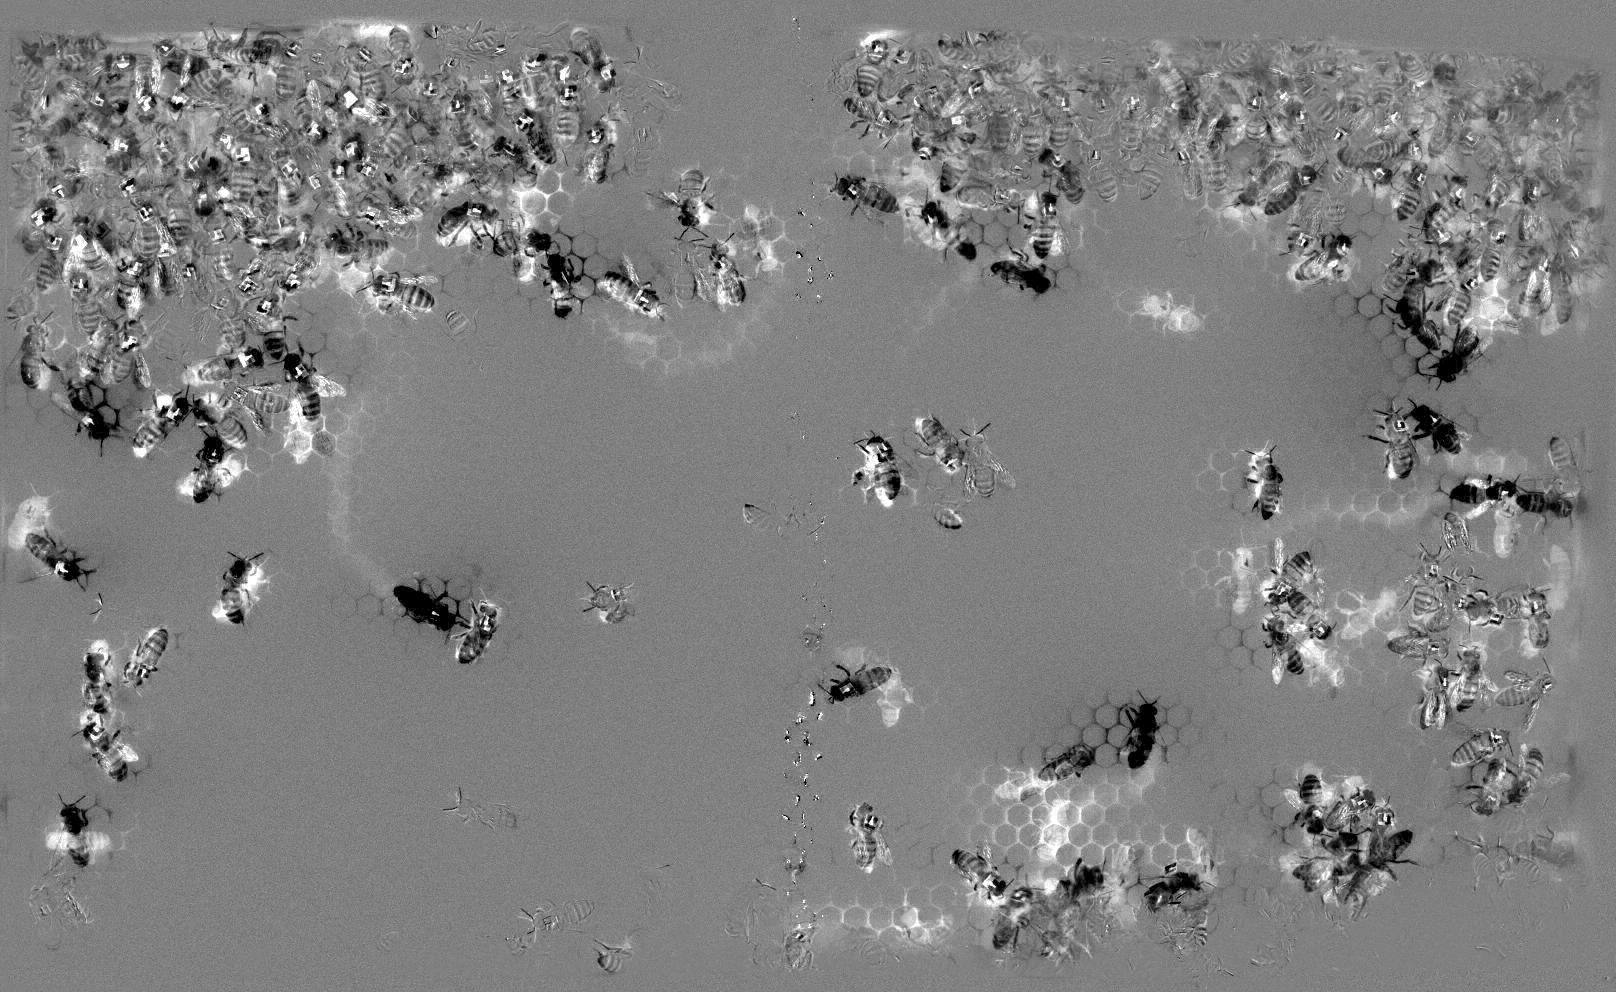
\includegraphics[width=0.85\textwidth]{figures/research/bees1.png}
\caption{\label{fig:bees} The result of a method for background subtraction, where only moving individuals are still visible.} 
\end{figure}

% GGG
\newpage
\item
\label{proj:fishslu}
\textbf{Fish Type Recognition in Underwater Videos for Sustainable Fishing}\\
Vladimir \' Curi\' c, Ida-Maria Sintorn\\
\ppartners{Arne Fj\"{a}lling, SLU Aqua, Stockholm}
\ffunding{Graduate School in Mathematics and Computing}
\aabstract{This projects investigates whether is possible to construct a system, which can determine the fish type using the underwater camera mounted in the tube at the end of the fishing trap (Fig. \ref{fig:fishslu}). The result of the image analysis will signal to the ramp at the end of the tube to either catch the fish or return the fish to a sea. Wild salmon are caught, bred, and planted back in the sea. To distinguish between wild and farmed salmon, each farmed salmon is marked by cutting off the adipose fin on the back of the salmon. Sustainable fishing is performed in a way that the farmed salmon should be caught, while the wild ones should be released back into the sea. The goal of the project is also to separate salmon from sea trout using texture and morphometric measurements.}

\begin{figure}[!htbp]
\centering
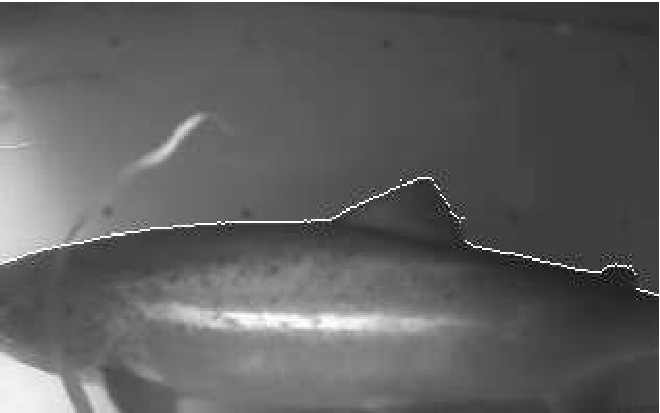
\includegraphics[width=0.6\textwidth]{figures/research/fritjof.pdf}
\caption{\label{fig:fishslu} Detecting adipose fin in salmon and sea trout.} 
\end{figure}

%HHH

\item
\label{proj:dipimage}
\textbf{DIPimage and DIPlib}\\
Cris Luengo\\
\ppartners{Bernd Rieger, Lucas van Vliet, Quantitative Imaging Group, Delft University of Technology, The Netherlands; Michael van Ginkel, Unilever Research and Development, Colworth House, Bedford, UK}
\ffunding{S-faculty, SLU}
\pperiod{0807--}
\aabstract{DIPimage is a MATLAB toolbox for scientific image analysis, useful for both teaching and research (\url{http://www.diplib.org}). It has been in active development since 1999, when it was created at Delft University of Technology. In 2008, when Cris Luengo moved to Uppsala, CBA was added to the project as a main development site. DIPlib, created in 1995, is a C library containing many hundreds of image analysis routines. DIPlib is the core of the DIPimage toolbox, and both projects are developed in parallel. Because DIPlib provides efficient algorithms, MATLAB is useful for image analysis beyond the prototyping stage. Together, MATLAB and DIPimage form a powerful tool for working with scalar and vector images in any number of dimensions. Version 2.5 was released in 2013, and improved the speed of image skew and rotation operations, the Fourier transform, and the reading of time series from disk; it also added some minor features and fixing some bugs. We also implemented the option to do arithmetic operations without changing the data type of the image, useful when working with very large images. This last change will appear in the next release.} 

% III

\item 
\textbf{UPPMAX Cluster Computing}\\
Martin Simonsson, Carolina W\"{a}hlby\\
\ppartners{Hans Karlsson, Elias Rudberg, Ola Spjuth, UPPMAX}
\ffunding{SciLife Lab Uppsala; eSSENCE; Dept.~of IT, UU}
\pperiod{1110-}
\aabstract{Life science applications generate a huge amount of image data that has to be stored and analysed in an efficient way. This project
is focused on providing easy access to high-performance computers and large-scale storage. In collaboration with Uppsala Multidisciplinary Center for Advanced Computational Science (UPPMAX) image analysis software are being installed and maintained on the cluster. Database solutions with easy web access to image data are also being developed and maintained. This project has also provided workshops and seminars to help life science researchers to get started and use the resources.In the end of 2013 we initiated our first large-scale image analysis project using the computer cluster working with 900 000 images from drug screening project.}

\clearpage

\end{enumerate}

%\end{document}

